\documentclass[11pt]{amsart}
\usepackage{float}
\usepackage{amsfonts, amstext, amsmath, amsthm, amscd, amssymb, upgreek}
\usepackage{bbm}
\usepackage{graphicx, color,  subfigure, wrapfig, overpic}
\usepackage{fullpage}
%\usepackage[all,cmtip]{xy} 
%\usepackage{tikz}
\usepackage{tikz-cd}
%\usepackage{mystyle}

\newcommand{\thmref}[1]{Theorem \ref{#1}}
\newcommand{\prpref}[1]{Proposition \ref{#1}}
\newcommand{\lemref}[1]{Lemma \ref{#1}}
\newcommand{\figref}[1]{Figure \ref{#1}}
\newcommand{\secref}[1]{Section \ref{#1}}
\newcommand{\remref}[1]{Remark \ref{#1}}
\newcommand{\eqnref}[1]{(\ref{#1})}
%\newcommand{\ref}[1]{Figure \ref{#1}}
\newcommand{\comment}[1]{}
\newcommand{\inv}{{-1}} % annoying to type {-1} when taking inverse


\textwidth 6.07in 
\textheight 8.6in 
\oddsidemargin 0.18in
\evensidemargin 0.18in
% \topmargin -0.07in
 
%%  If the following line is uncommented, we see the labels of theorems, figures, etc. in the margins.
% \usepackage[notref,notcite]{showkeys}
\setlength{\marginparwidth}{0.8in}
\let\oldmarginpar\marginpar
\renewcommand\marginpar[1]{\oldmarginpar[\raggedleft\footnotesize #1]%
{\raggedright\footnotesize #1}}

%This command stops the Math Review numbers appearing in the references! 
\AtBeginDocument{
   \def\MR#1{}
}
\newcommand{\Sp}{{S}}
\newcommand{\C}{\mathbb{C}}
\newcommand{\R}{\mathbb{R}}
\newcommand{\Q}{\mathbb{Q}}
\newcommand{\Z}{\mathbb{Z}}
\newcommand{\N}{\mathbb{N}}
\newcommand{\CC}{\mathbb{C}}
\newcommand{\RR}{\mathbb{R}}
\newcommand{\HH}{\mathbb{H}}
\newcommand{\ZZ}{\mathbb{Z}}
\newcommand{\bfloor}[1]{\left\lfloor #1\right\rfloor}
\renewcommand{\P}{\mathcal P}
\newcommand{\A}{\mathcal A}
\newcommand{\W}{\mathcal W}
\newcommand{\vol}{{\rm vol}}
\newcommand{\cut}{{\backslash \backslash}}
\newcommand{\bdy}{\partial}
\newcommand{\voct}{{v_{\rm oct}}}
\newcommand{\vtet}{{v_{\rm tet}}}
\renewcommand{\L}{\mathcal L}
\newcommand{\cp}{\mathcal{C}}
\newcommand{\toF}{{\overset{F}{\longrightarrow}}}
\newcommand{\K}{\upkappa}

\def\co{\colon\thinspace}


\newcommand{\torus}{{\mathbb{T}^2}}
\newcommand{\sT}{{\mathcal{T}}}
\newcommand{\cD}{{\mathcal{D}}}
\newcommand{\cL}{{\mathcal{L}}}



\newcommand{\RRR}{{\underline{\mathfrak{R}}}}
\newcommand{\QQQ}{{\underline{\mathfrak{Q}}}}
\newcommand{\CCC}{{\underline{\mathfrak{C}}}}
\newcommand{\PPP}{{\underline{\mathbf{\Phi}}}}
\newcommand{\TTT}{{\underline{\mathbf{\Theta}}}}
\newcommand{\LLL}{{\underline{\mathfrak{L}}}}

\newcommand{\cev}[1]{\overset{\leftarrow}{#1}}

\newcommand{\del}{\partial}
\newcommand{\ddd}[1]{{\frac{\del}{\del #1}}}
\newcommand{\vphi}{\varphi}
\newcommand{\veps}{\varepsilon}
\newcommand{\llong}{{\text{long}}}
\newcommand{\Span}{{\text{span}}}
\newcommand{\Pol}{{\text{Pol}}}
\newcommand{\toruscomp}[1]{{\torus \times I - #1}}

\theoremstyle{plain}
\newtheorem{theorem}{Theorem}[section]
\newtheorem{corollary}[theorem]{Corollary}
\newtheorem{lemma}[theorem]{Lemma}
\newtheorem{prop}[theorem]{Proposition}
\newtheorem{claim}[theorem]{Claim}
\newtheorem{conjecture}[theorem]{Conjecture}
\newtheorem{example}[theorem]{Example}

\newtheorem*{namedtheorem}{\theoremname}
\newcommand{\theoremname}{testing}
\newenvironment{named}[1]{\renewcommand{\theoremname}{#1}\begin{namedtheorem}}{\end{namedtheorem}}
\theoremstyle{definition}
\newtheorem{define}[theorem]{Definition}
\newtheorem{definition}[theorem]{Definition}
\newtheorem{question}[theorem]{Question}
\newtheorem{remark}[theorem]{Remark}

\title{Hyperbolicity of Augmented Links in the Thickened Torus}


\author[Alice Kwon and Ying Hong Tham]{Alice Kwon and Ying Hong Tham}


\begin{document}
\maketitle

\begin{abstract}
For a hyperbolic link $K$ in the thickened torus,
we show there is a decomposition of the complement of a link $L$,
obtained from augmenting $K$, into torihedra. We further decompose 
the torihedra into angled pyramids and finally angled tetrahedra.
These fit into an angled structure on a triangulation of the link complement,
and thus by \cite{Casson-Rivin}, this shows
that $L$ is hyperbolic.  
\end{abstract}

\section{Introduction}
\label{s:intro}

Given a twist-reduced diagram of a link $K$, \emph{augmenting} is a process in
which an unknotted circle component (augmentation) is added to one or more twist
regions (a single crossing or a maximal string of bigons) of $K$.
%%By a standard argument using a Dehn twist
%%on the complement of the crossing circle,
%%the added circle component allows us to remove full twists
%%(i.e. pairs of bigons)
%%at the twist region of $K$
%%while keeping the link complement the same.
%%If the twist region has an odd number of crossings,
%%then all but one crossing is removed,
%%whereas if the twist region has an even number of crossings,
%%then all are removed.
%We can remove full twists by a standard argument using a Dehn twist 
%on the complement of the crossing circle.
The newly obtained link is called an 
\emph{augmented link} and the newly obtained diagram is called an 
\emph{augmented link diagram}. See Figure
\ref{fig:Augmentations}. 


Adams showed in \cite{CA} that given a hyperbolic alternating link $K$ in
$\Sp^3$ the link $L$ obtained by augmenting $K$ is hyperbolic. In this paper we
investigate if this statement holds for links in the thickened torus i.e. if $L$
is a link obtained from augmenting a hyperbolic alternating link $K$ in the
thickened torus. We define augmenting similarly for links in the thickened torus
with their associated link diagram on $\torus \times \{0\}.$ 


Menasco \cite{Menasco} showed that there are decompositions
of the complements of alternating links in $\Sp^3$
into two topological polyhedra,
a top polyhedron and a bottom polyhedron.
For alternating links $K$ in the thickened torus,
Champanerkar, Kofman and Purcell \cite{CKP2}
showed that there is a decomposition of the
complement of $K$ into objects called torihedra, which we think of as
counterparts to Menasco's decomposition % of links in $\Sp^3$ into polyhedra,
for links in the thickened torus;
just like Menasco's decomposition, one obtains a top and a bottom torihedron.


In \secref{s:auglinks} we show that for augmented
links in the thickened torus (not necessarily fully augmented),
one can also obtain a decomposition of the
complement into a top and bottom torihedron.
In \secref{s:hyperbolicity}, we prove that
many augmented alternating links in the thickened torus are hyperbolic.


We point out that \cite{kwon2020fully}, the first author
proved that \emph{fully} augmented links in the thickened torus
are hyperbolic, so this paper can be seen as a generalization
of that work.


While revising this paper, we learned that \cite{adams2021generalized}
proves a generalization of our work here,
showing hyperbolicity of generalized augmented links
in an arbitrary thickened surface.
We note that our approach, based on angle structures,
is different from theirs, which is based on topological arguments.



\begin{figure}
\centering  
\begin{tabular}{cc}
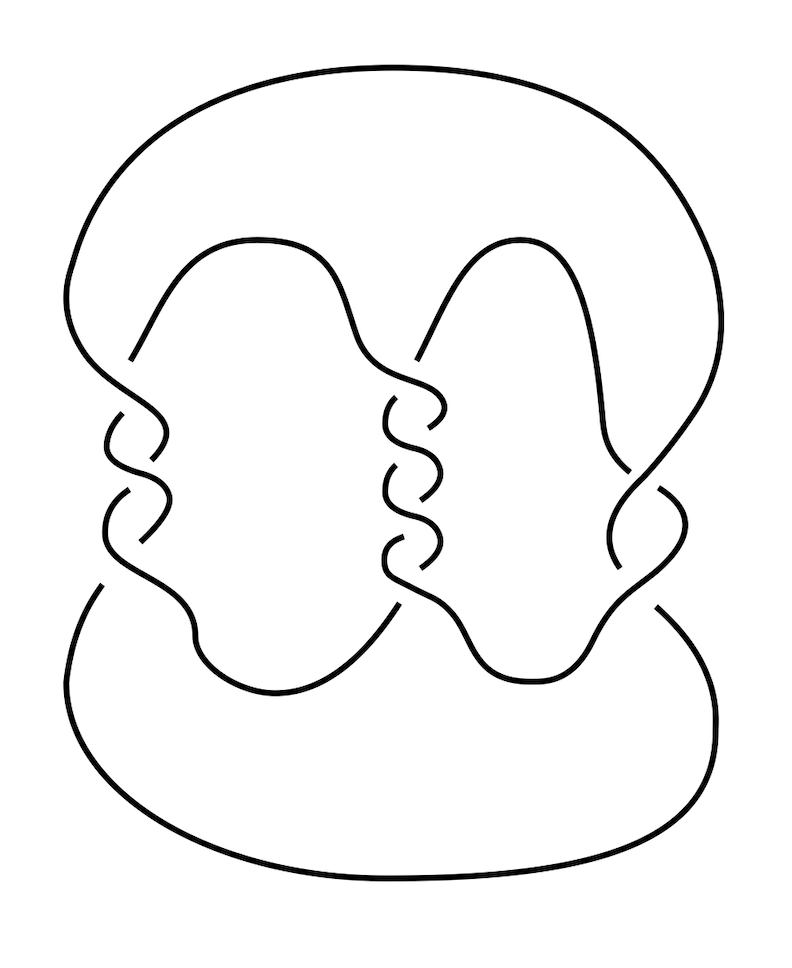
\includegraphics[height=4cm]{augmentation1.png}
\;\;\;\;
& 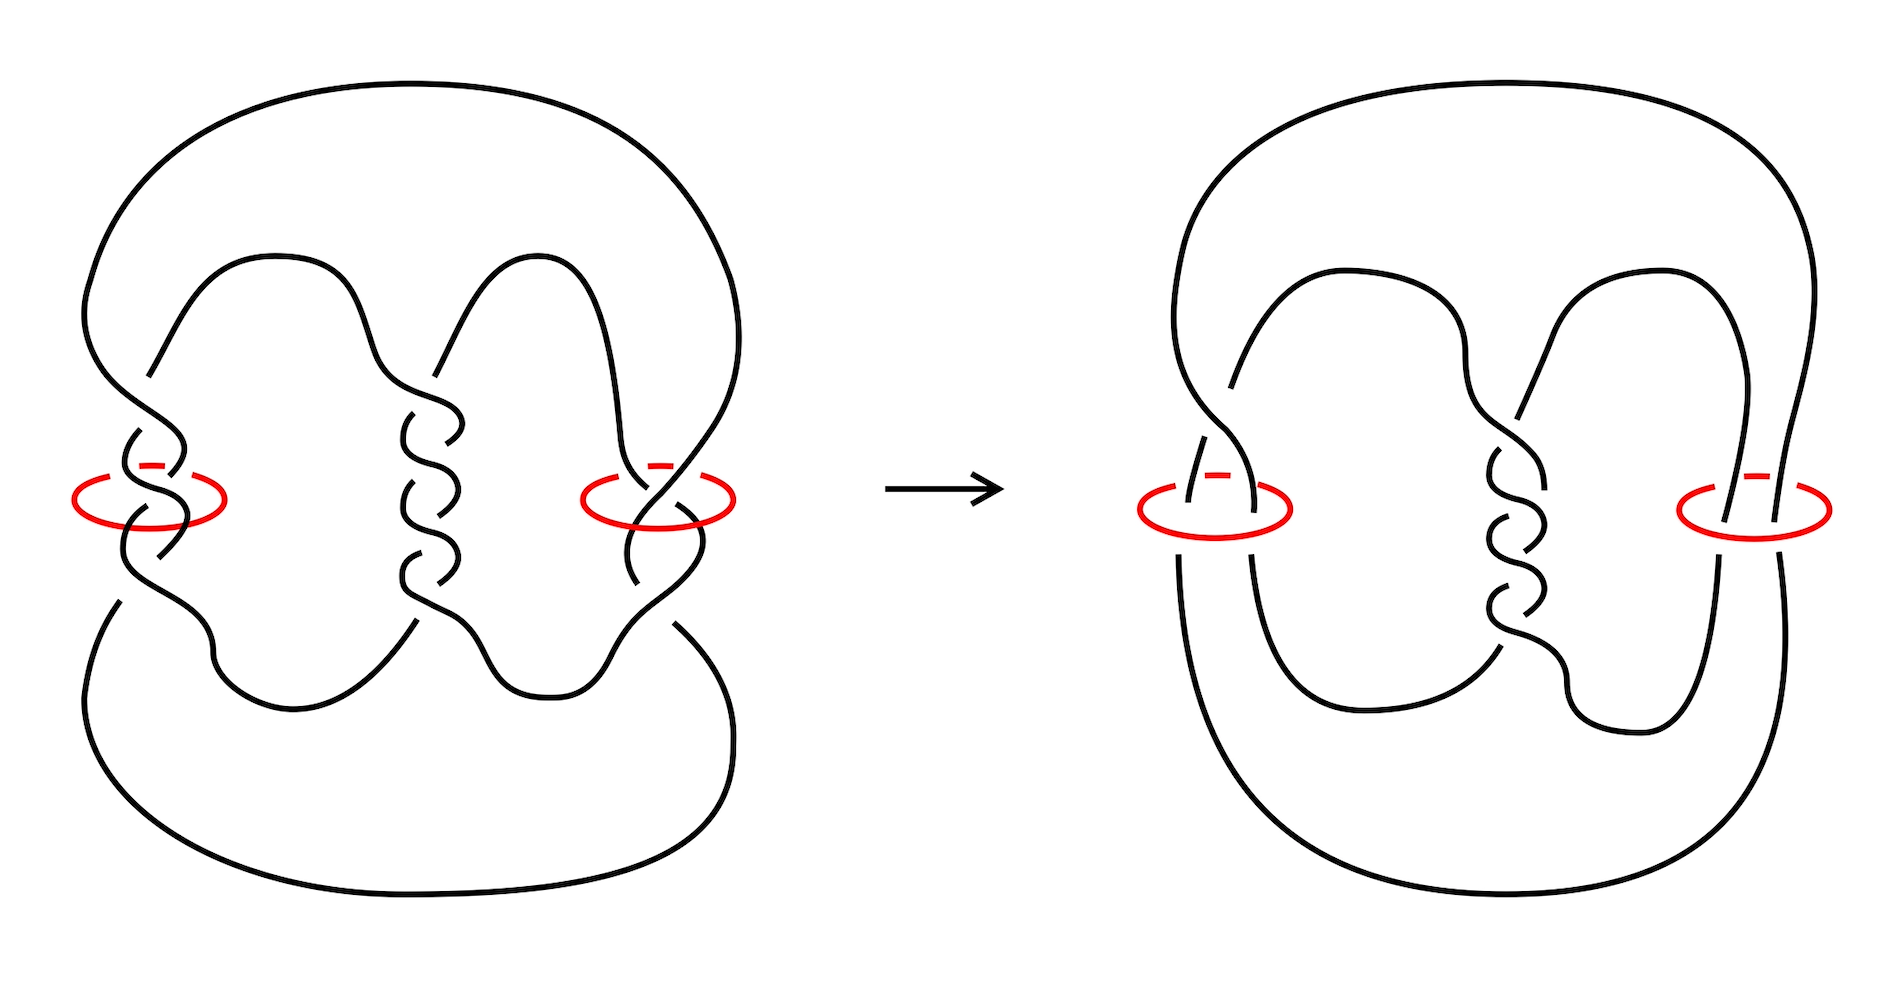
\includegraphics[height=4cm]{augmentation2.png}
\\
(a)
& (b)
\end{tabular}
\caption{(a) pretzel knot before augmentation
(b) pretzel knot after augmentation;
second diagram shows
removal of full twists in the augmented twist regions.}
\label{fig:augmentationS3}
\end{figure}
 
 
 %%%%%%%%%%%%%%%%%%%%%%%%%%%%%%%%%%%%%%%%%%%%%%%%%%%%%%%% 
\section{Augmented Links}
\label{s:auglinks}

TODO Notation section: $I = (-1,1)$.

Champanerkar, Kofman and Purcell have studied alternating links in the thickened
torus \cite{CKP2}. They define a link in the thickened torus as a quotient of a
biperiodic alternating link as follows:
 
\begin{define}
\label{def:biperiodiclink}
A \emph{biperiodic alternating link} $\cL$ is an infinite link
in $\R^2 \times I$ with a link diagram $\cD \subset \R^2$
such that $\cL$ and $\cD$ are
invariant under the action of a two dimensional lattice $\Lambda$
on $\R^2$ by translations.


The quotient $L=\mathcal{L}/\Lambda$ is an alternating link in
the thickened torus $\torus \times I$,
whose projection onto $\torus \times \{0\} = \R^2 \times \{0\} /\Lambda$
is an alternating link diagram $\cD/\Lambda$.
\end{define}


We refer to $\torus \times \{0\}$ as the \emph{projection plane}.


\begin{remark}
Since $\torus \times I \cong \Sp^3 - H$, where $H$ is a Hopf link.
The complement $\torus \times I- L = \Sp^3 - (L \cup H)$.
\end{remark}

Champanerkar, Kofman and Purcell \cite{CKP2} extended
the definition of prime links in $\Sp^3$
for links in $\torus \times I$ called weakly prime. 

\begin{define} \label{def:weaklyprime}
A diagram $D \subset \torus$
of a link $L$ in the thickened torus $\torus \times I$
is \emph{weakly prime}
if whenever a disk is embedded in $\torus$
meets the diagram transversely in exactly two edges,
then the disk contains a simple edge of the diagram and no crossings.
\end{define}


\begin{define}
Recall that a \emph{twist region}
in a link diagram is a maximal sequence of vertices
such that consecutive vertices are two vertices of a bigon face,
and consecutive bigons meet only at a vertex (not an edge).
\footnote{There is an ambiguity of ``maximality'' in this definition:
for example, if a vertex of a link diagram meets exactly one bigon,
it can be considered as part of a twist region of length 2
(given by that bigon),
or it can be considered as part of a twist region of length 1,
as there are no bigons in the other ``direction''.
It should be clear which ``direction'' a twist region is going
when we deal with augmentations later.
}
For links in the thickened torus,
a \emph{twist region} in a link diagram of $L=\mathcal{L}/\Lambda$ in $\torus
\times I$, is the quotient of a twist region in the biperiodic link
$\mathcal{L}$. 


A biperiodic link
$\mathcal{L}$ is called \emph{twist-reduced} if for any simple closed curve on
the plane that intersects the diagram of $\mathcal{L}$
transversely in four points, with two
points adjacent to one crossing and the other two points adjacent to another
crossing, the simple closed curve bounds a subdiagram consisting of a (possibly
empty) collection of bigons strung end to end between these crossings. We say
the diagram of $L$ is \emph{twist-reduced}
if it is the quotient of a twist-reduced biperiodic
link diagram.
\end{define}


We note that when a link diagram is cellular
(Definition \ref{d:cellular}),
a twist region in the torus cannot be a cycle;
otherwise, the face adjacent to the twist region would be an annulus.


Now we can define augmentation for a link in $\torus \times I$ the same way we
define augmentation for links in $\Sp^3$:
%For a link in $\torus \times I$, the
%crossing circles are added to the diagram projected onto $\torus \times \{0\}$.
%Let $D(L)$ be a twist-reduced diagram of a link $L$ in $\torus \times I$, we define
%\emph{augmenting} as a process in which an unknotted circle component is added
%to one or more twist regions of $D(L)$. See Figure \ref{fig:Augmentations}

\begin{definition}
Let $D(K)$ be a twist-reduced diagram of a link $K$ in $\torus \times I$.
We define
\emph{augmenting} as a process in which an unknotted circle component,
called a \emph{crossing circle},
is added to one or more twist regions of $D(K)$
(see Figure \ref{fig:Augmentations});
we call the resulting link $L$ an \emph{augmented link obtained from $K$}.
We say $L$ is \emph{fully} augmented if $L$ is obtained by augmenting
$K$ at \emph{every} crossing/twist site.
\label{d:augmentation}
\end{definition}


As pointed out in the introduction,
after augmenting a twist region,
a standard Dehn twist argument allows us to remove
a full twist (that is, two bigons).

\begin{definition}
We say an augmentation has a \emph{half twist}
if at least one of the augmented twist regions
has an odd number of vertices (i.e. even number of bigons).
\label{d:half-twist}
\end{definition}



\begin{definition}
A graph $G = (V,E)$ on the torus is \emph{cellular}
if its complement is a collection of open disks.
\label{d:cellular}
\end{definition}

%We say that a link diagram in the thickened torus is
%\emph{cellular}.

%%\begin{remark}
%%If $L$ is augmented at \emph{every} crossing/twist site we say $L$ is \emph{fully} augmented.
%%\end{remark}


\begin{figure}
\centering
\begin{tabular}{cccc}
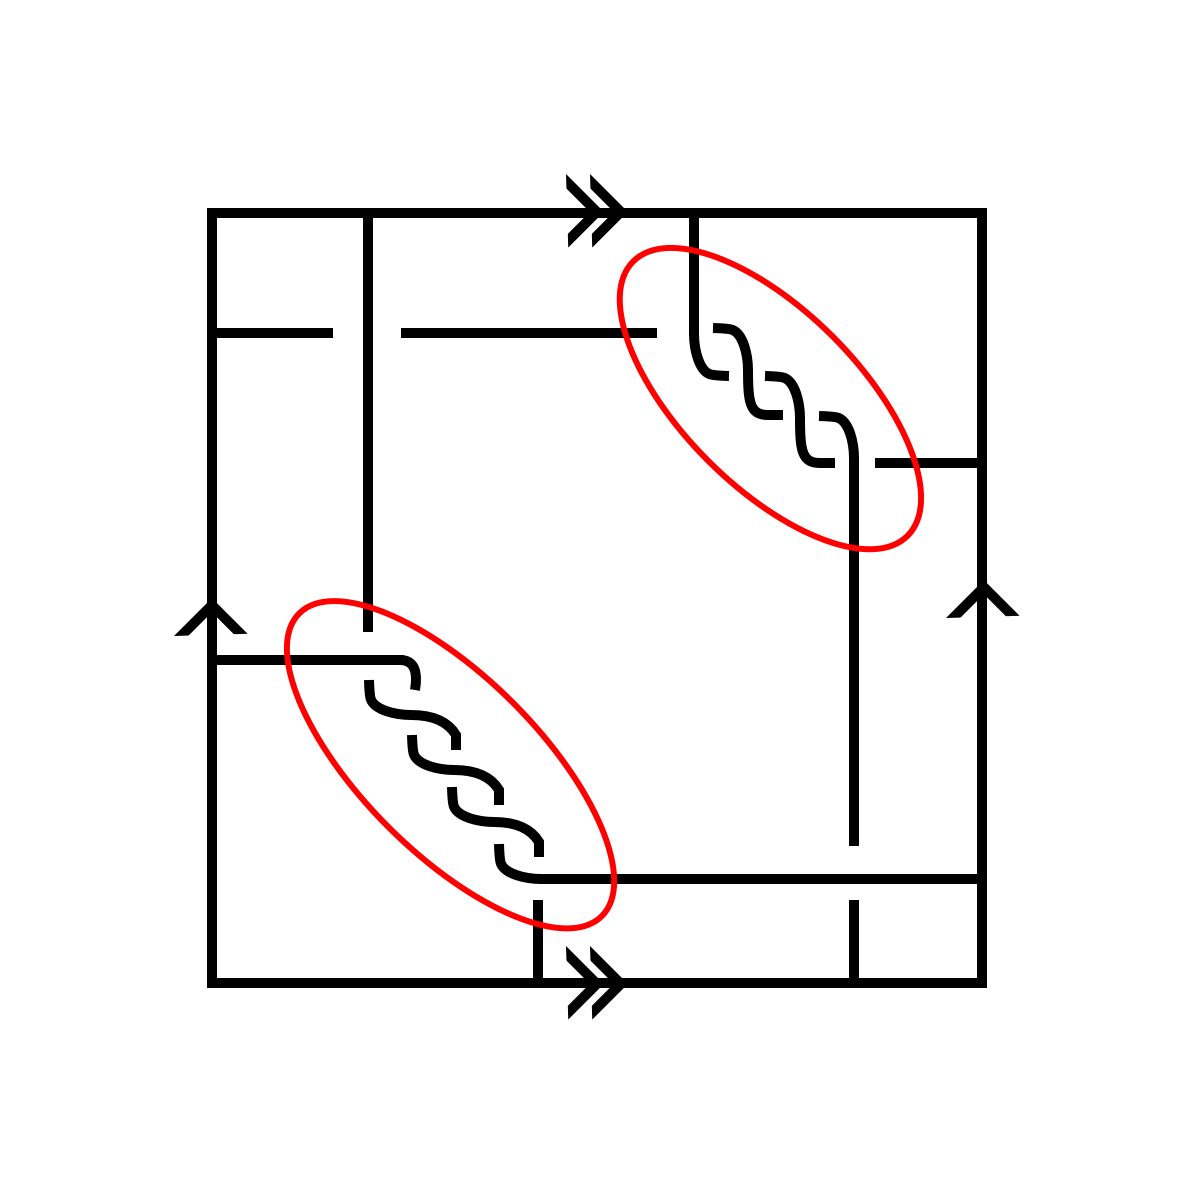
\includegraphics[width=3cm]{fig1.png}&
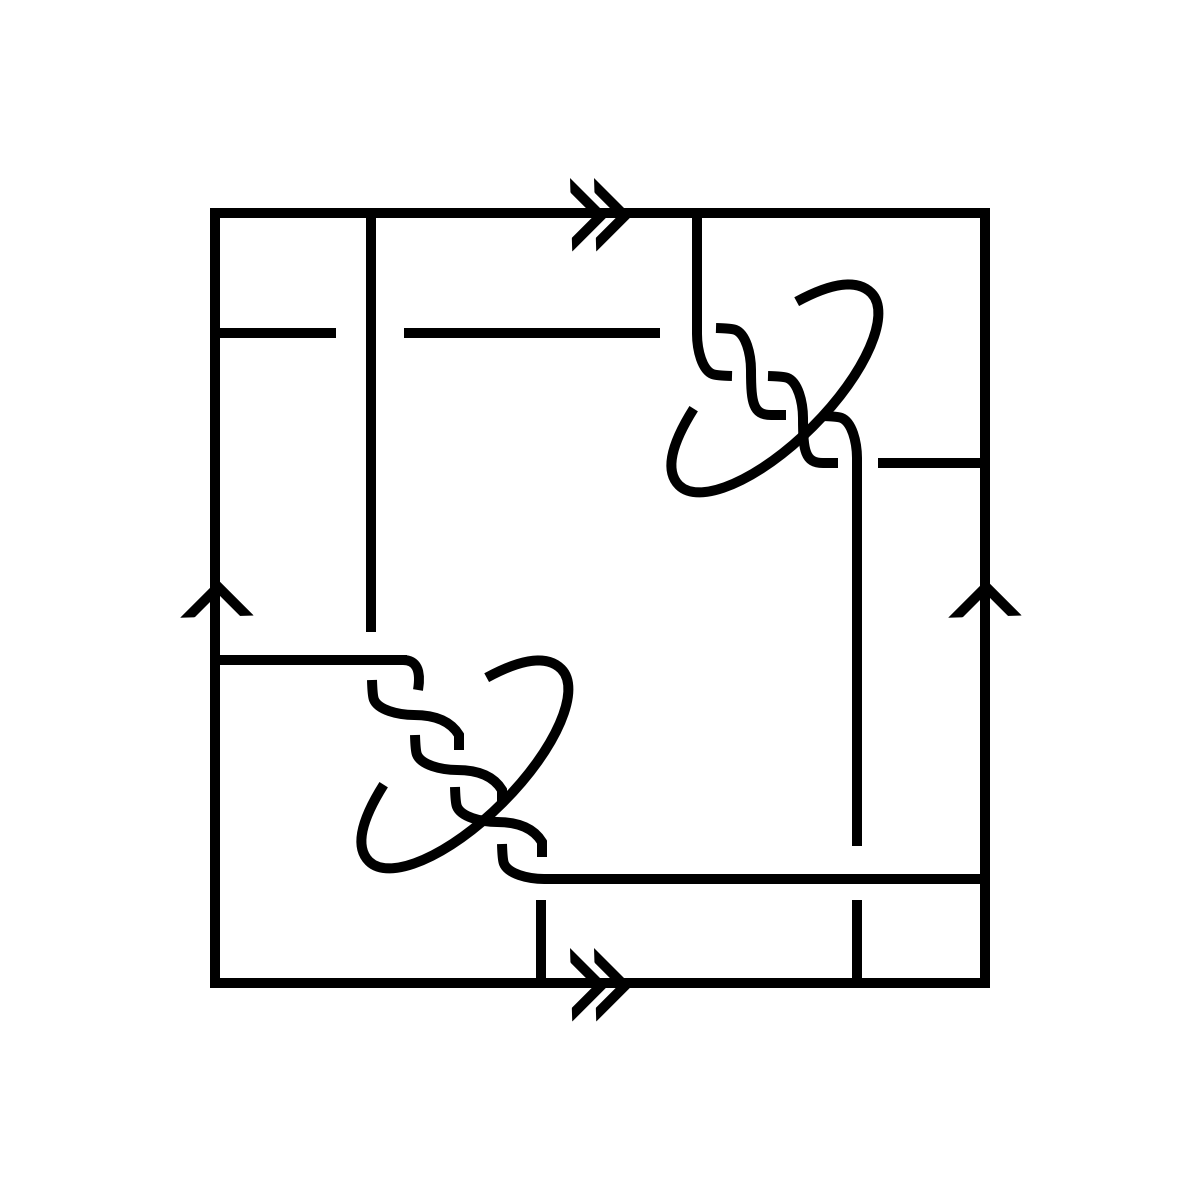
\includegraphics[width=3cm]{twist-augment.png}&
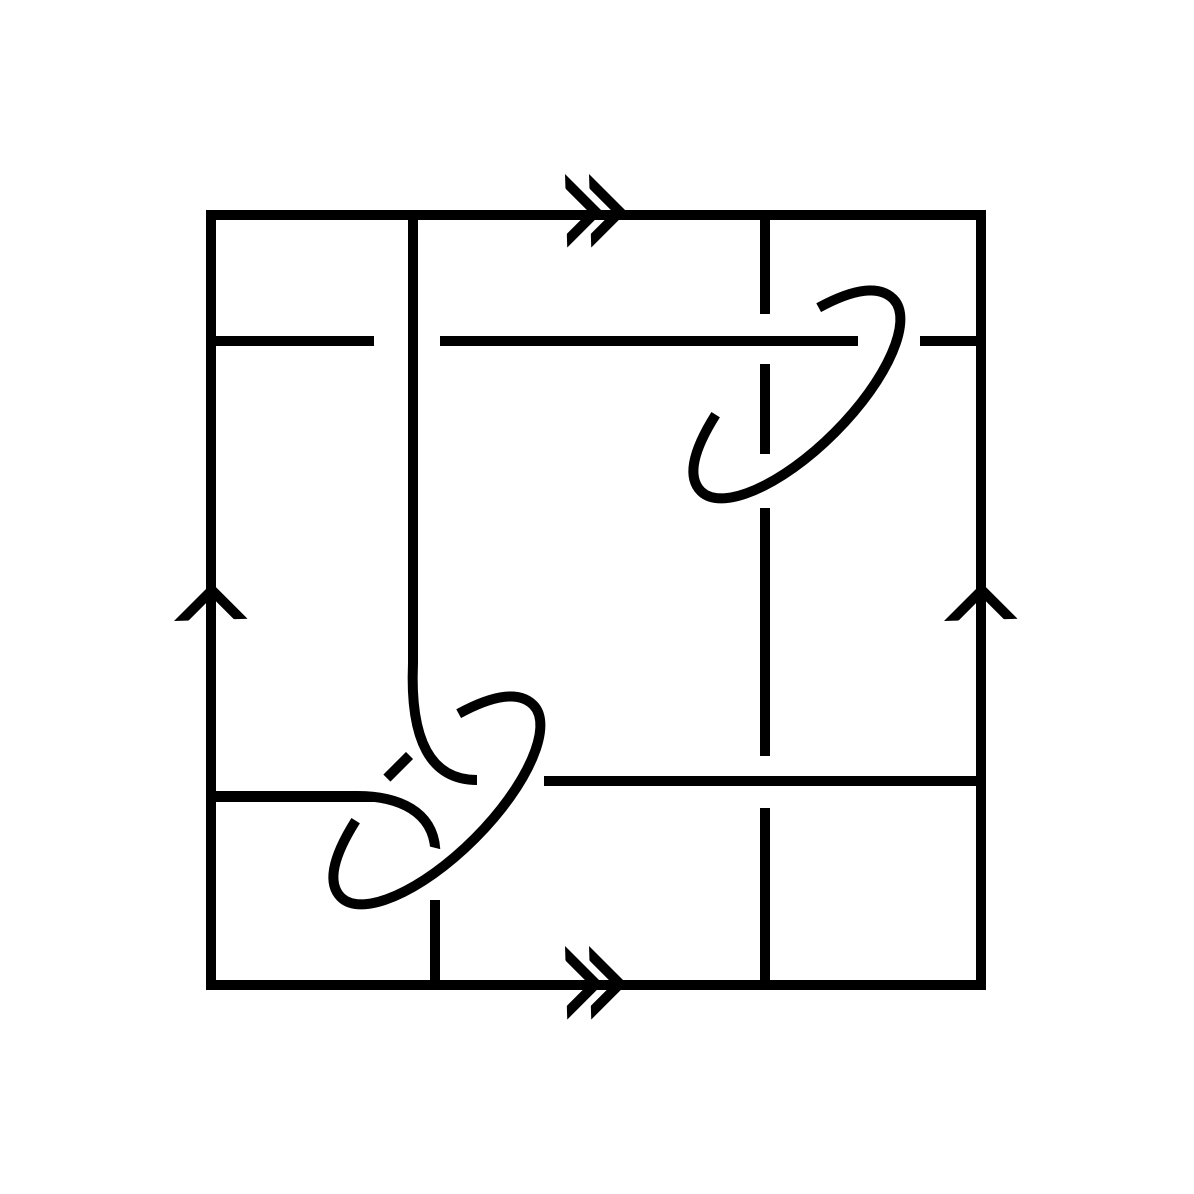
\includegraphics[width=3cm]{fig-2.png}\\
 % 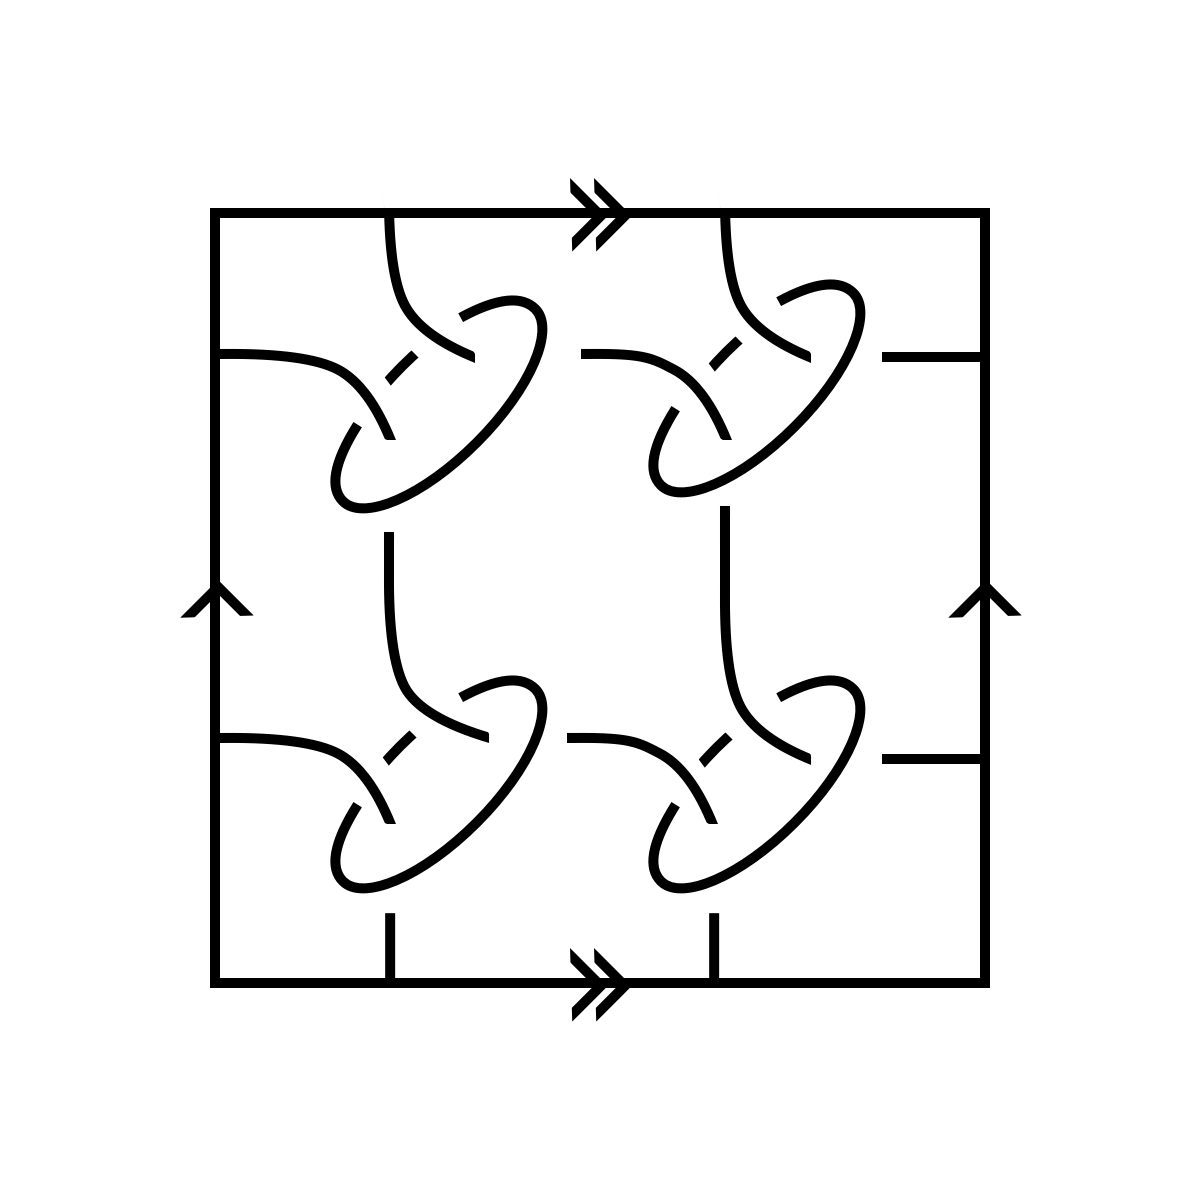
\includegraphics [width=3cm]{fal}\\
A&B&C
\end{tabular}
	 \caption{A: The top right has an odd number of twists while the bottom left has
	 an even number of twists. B: The picture of the link on the right after
	 augmentation twist regions circled in red. C: The link with full twists
	 removed.}
\label{fig:Augmentations}
\end{figure}
%%%%%%%%%%%%%%%%%%%%%%%%%%%%%%%%%%%%%%%%%%%%%%%%%%%% 

\subsection{Torihedral Decomposition of Augmented Alternating Links in Thickened Torus}


We present a method of decomposing an augmented link
(not necessarily fully augmented) in the thickened torus into
objects called ``torihedra'' as defined below.
Decomposing alternating links in the thickened torus into 
torihedra were first described in \cite{CKP2},
then later used for fully augmented links in 
the thickened torus in \cite{kwon2020fully}.
The idea is to combine methods of Menasco
\cite{Menasco} and the use of crossing edges
between (TODO for?) each crossing of our link
and Lackenby's ``cut-slice-flatten" method \cite{lackenby}
on the augmentation
sites.



\begin{define}\cite{CKP2}
\label{def:torihedron}
A \emph{torihedron} $\sT$ is a cone on the torus, 
i.e. $\torus \times [0,1]/(\torus \times \{1\})$, with a cellular graph
$G = G(\sT)$ on $\torus \times \{0\}$.
The \emph{ideal torihedron} $\sT^\circ$ is $\sT$ with the
vertices of $G$ and the vertex $\torus \times \{1\}$ removed. Hence, an ideal
torihedron is homeomorphic to $\torus \times [0,1)$ with a finite set of points
(ideal vertices) removed from $\torus \times \{0\}$.
We refer to the vertex $\torus \times \{1\}$ as the \emph{cone point}
of $\sT$.
\end{define}


For visualization purposes, we typically draw the graph $G(\sT)$ of a
torihedron from the perspective of the cone point $\torus \times \{1\}$.
Note however that later we will be dealing with
``top'' and ``bottom'' torihedra that are glued together
along their torus boundary faces;
to avoid confusion, we will visualize the graphs of both torihedra
from the perspective of the cone point of the ``top'' torihedron.


If the faces of $G(\sT)$ are disks,
then $\sT$ can be decomposed into a union of pyramids,
obtained by coning each face to the cone point of $\sT$.
This also gives a decomposition of the corresponding ideal torihedron
$\sT^\circ$ into ideal pyramids.
We call these the \emph{pyramidal decompositions} of $\sT$ and $\sT^\circ$.


\begin{definition}
Let $G$ be a graph on the torus.
Let $v$ be a vertex and $e,e'$ be distinct edges that meet $v$.
A \emph{left (resp. right) bow-tie modification to $v,e,e'$}
is the process of removing $v,e,e'$ and adding in a ``bow-tie''
as in Figure \ref{TODO} (a) (resp. (b)).
We call the TODO long edges, the TODO short edges,
and TODO diagonal edges.
TODO in figure caption, left bow-tie modification so-called because
the triangular face appears to the left of the long edges;
also note that left/right conincide with Figure \ref{f:right_left_aug}
\label{d:diagram-bowtie}
\end{definition}


\begin{define}
We say a twist region is \emph{right-augmented} if, when both strands are
(locally) oriented so that they cross the augmentation disk in the same
direction, the crossing is a positive right-handed half-twist.
We say a twist is \emph{left-augmented} if it is not right-augmented.
See Figure \ref{f:right_left_aug}.
\end{define}

\begin{figure}
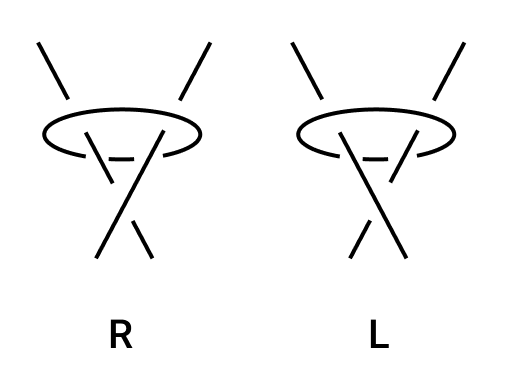
\includegraphics[width=5cm]{more_pictures/right_left_aug.png}
\caption{R: right augmentation, L: left augmentation}
\label{f:right_left_aug}
\end{figure}

We can recover $L$ from the link diagram of $K$
together with labels at vertices indicating left- or right-augmentation.


\begin{prop}\label{p:tori_decomp}
Let $K$ be an alternating link in the thickened torus
with a cellular link diagram,
and let $L$ be an augmented link obtained from $K$.
%Let $G(L)$ be a diagram of the link on $\torus \times \{0\}$.
There is a decomposition of the complement,
$(\torus \times I) - L$, into two ideal torihedra.
\end{prop}


\begin{proof}
We first give a description of the topological operations
that give the torihedral decomposition;
this will justify the 
more concise description purely in terms of link diagrams
which we present at the end.


We will begin by assuming that $L$ has no half twists.
Let $L = K \cup C$, with $C$ being the collection of crossing circles.
%Arrange the link diagram of $L$ in the following way:
Arrange $L$ in the following way:
place the circle components in $C$ perpendicular to
the projection plane $\torus \times \{0\}$,
and leave the remaining part of the link $K \subseteq L$
lying in the projection plane (except at crossings of $K$).
Thus, the projection of $L$ onto the projection plane
will be a diagram $D(K)$ of $K$
together with line segments corresponding to crossing circles.
(We demand that $D(K)$ be alternating and twist-reduced.)
As discussed before, we may remove full twists (i.e. pairs of bigons)
from the twist regions of $K$ that are augmented in $L$,
and since $L$ is assumed to have no half twists,
the two edges of $D(K)$ that go through a crossing circle
do not meet (see Figure \ref{fig:Augmentations} C).
From now on, we will take $K$ to be this modified link
(with full twists removed).


We now place a \emph{crossing edge} at each crossing of $K$,
connecting the top and bottom strands at the crossing
(see Figure \ref{fig:crossingArc} (a)).
%so that for each crossing edge,
%one end of the edge lies on a bottom strand while the other
%end lies on a top strand as in Figure \ref{fig:crossingArc} (a).

\begin{figure} 
\centering 
\begin{tabular}{cc}
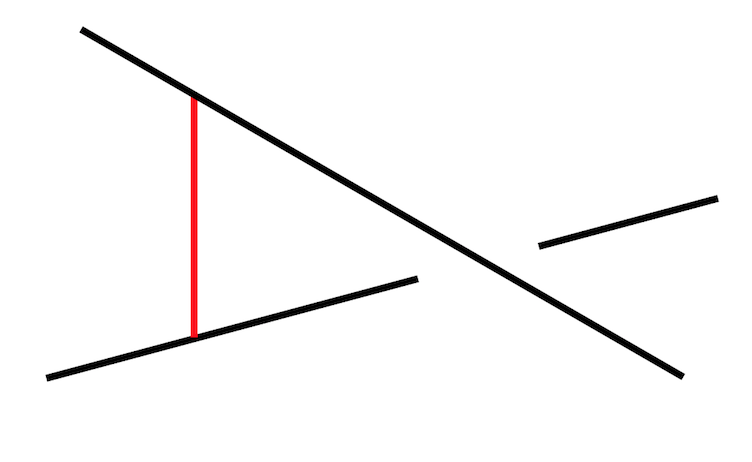
\includegraphics[width=4cm]{crossingArc.png}
& 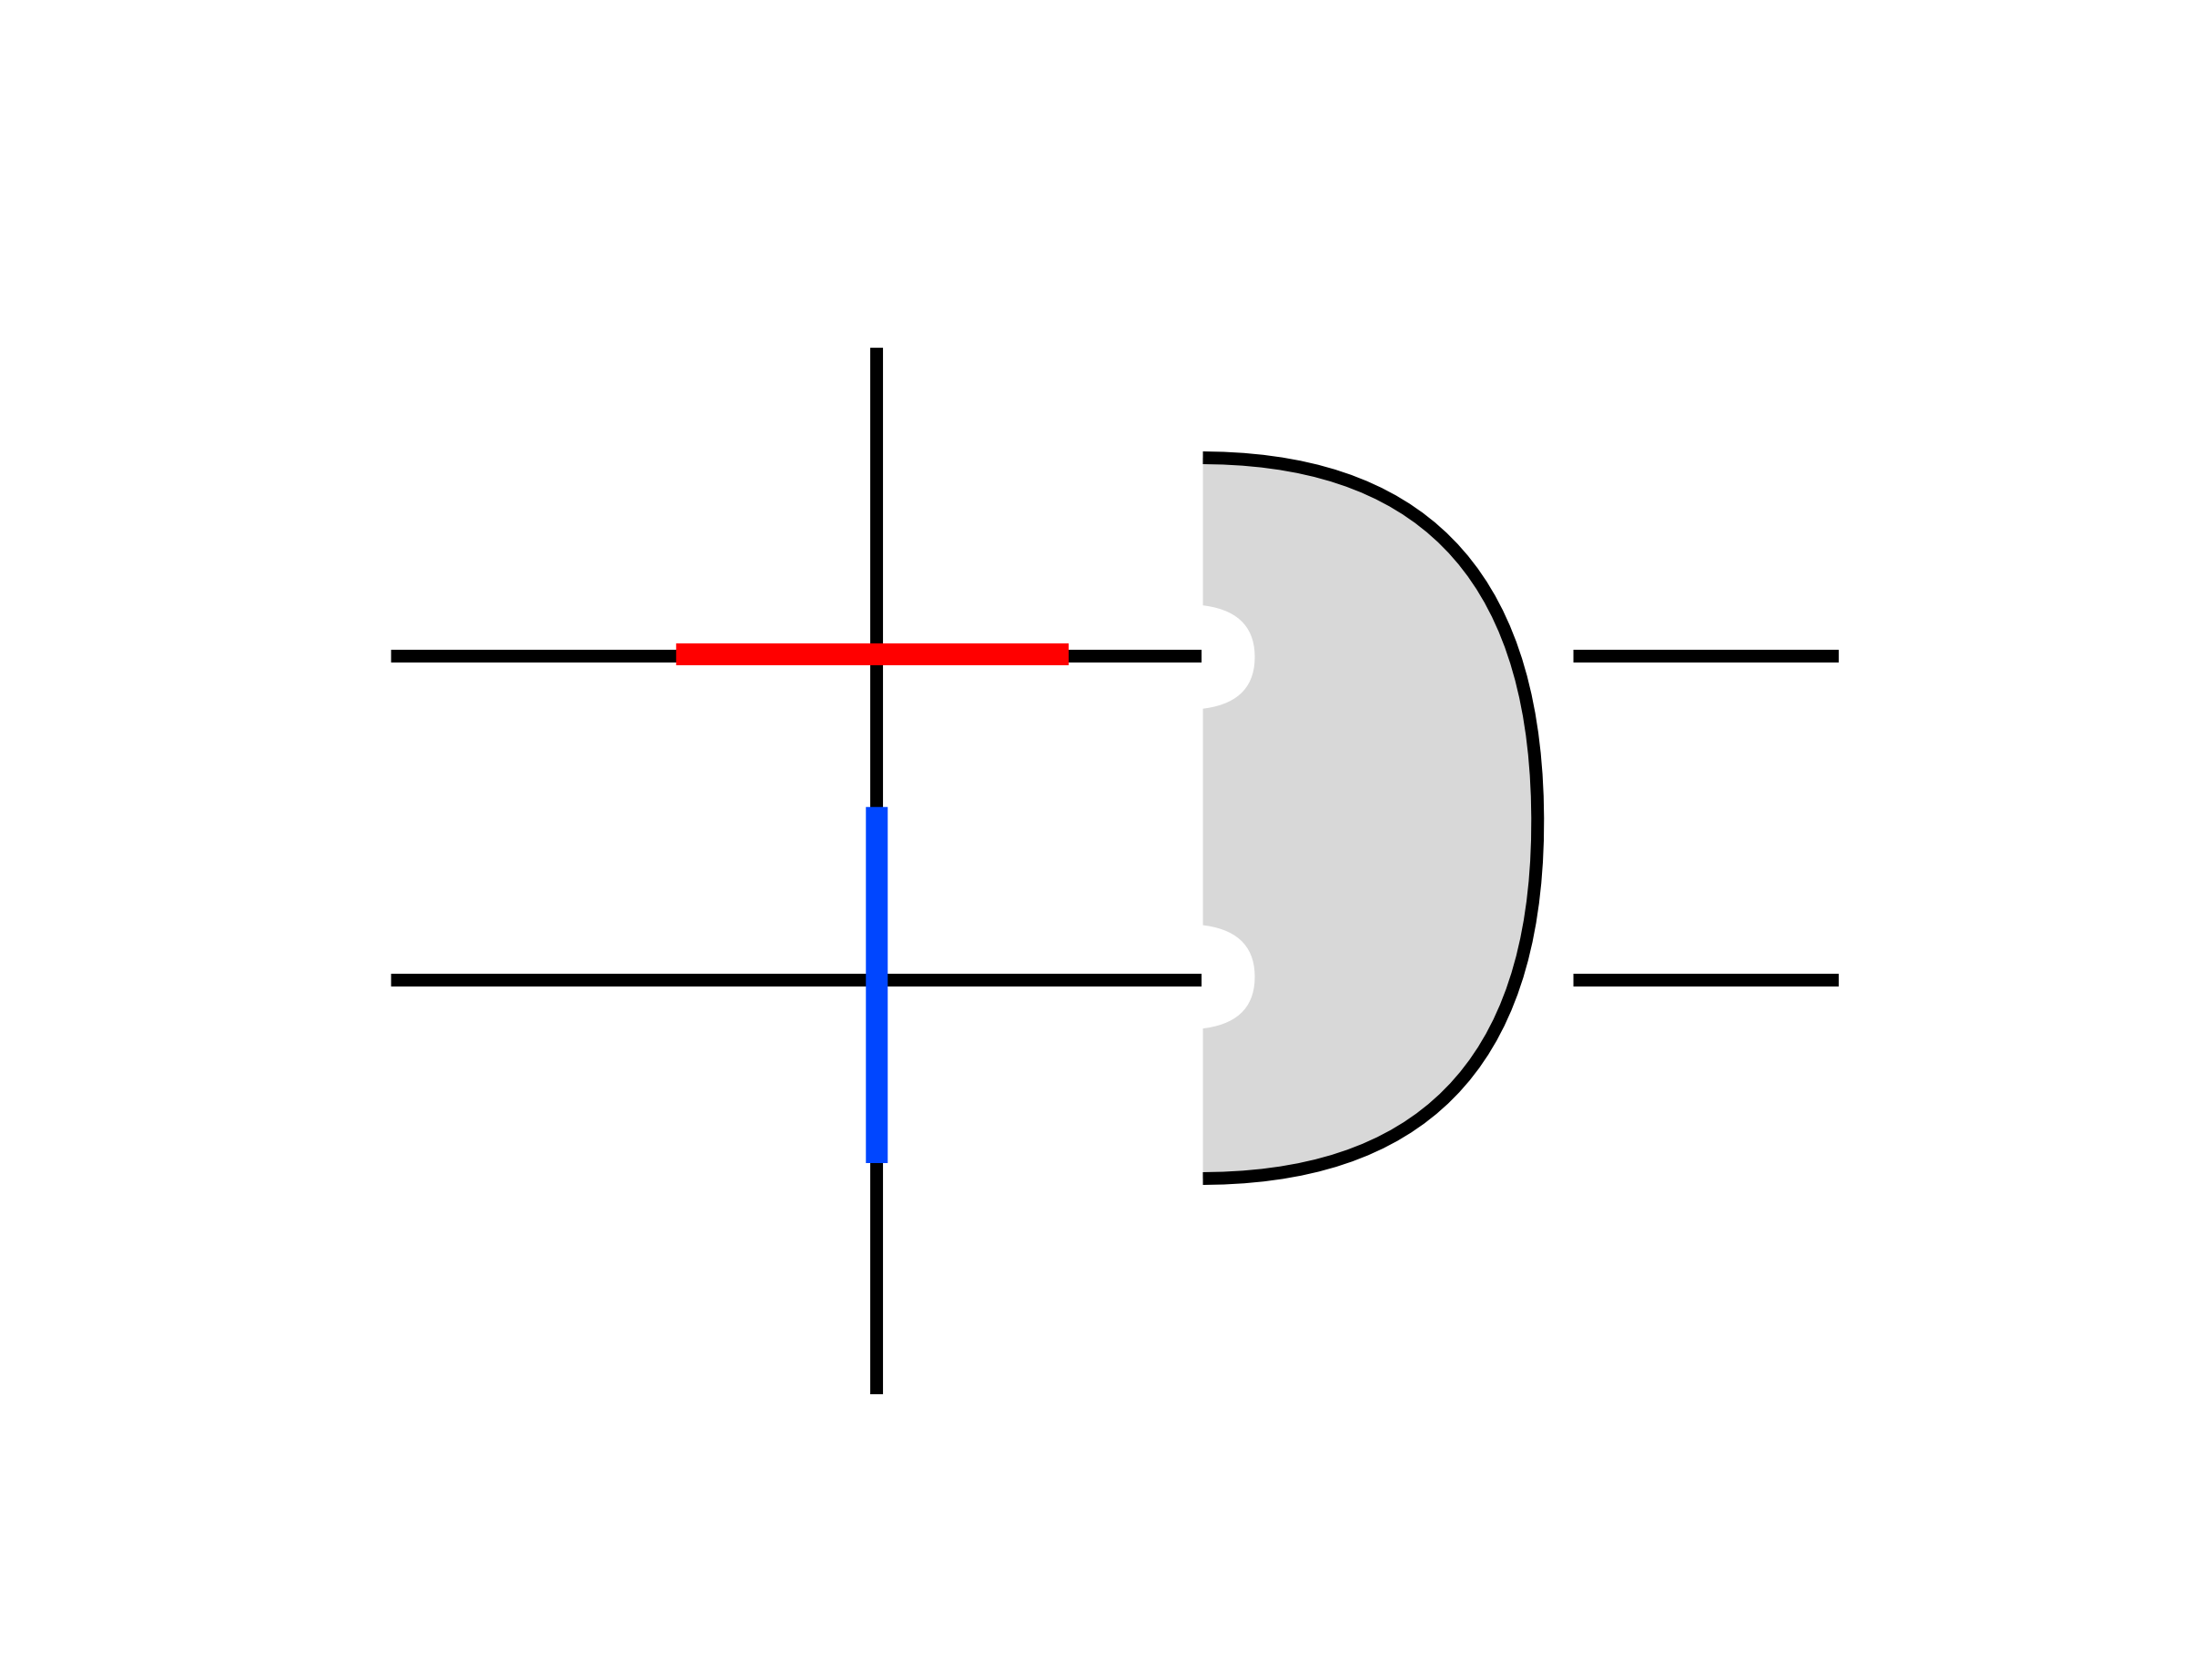
\includegraphics[width=5cm]{crossingPush.png}
\\
(a)
& (b)
\end{tabular}
\caption{(a) The black strands are
part of the link and the red strand is the crossing edge.
(b) The blue and
red edges represent the split crossing edges and the shaded half disk is bounded
by the crossing circle} 
\label{fig:crossingArc} 
\end{figure}


Next we construct the graph that will define the ``top'' torihedron.
We view the link from the point at infinity from the top end
($\torus \times \{1\}$) of the thickened torus.
At each crossing of $K$,
push the top strand towards the bottom strand,
splitting the crossing edge into two
identical edges and spreading them apart
as in Figure \ref{fig:crossingArc} (b).
%We push the link
%components to infinity and stretch the crossing edge so that we have flattened
%the link onto $\torus \times \{0\}$ except for the crossing circles,
%which remains perpendicular to the projection plane. 
 

%Now place a disk on each crossing circle, so that the disk is bounded by
%the crossing circle.
Now for each crossing circle $c$, consider a spanning disk $B_c$;
$B_c$ intersects the projection plane $\torus \times \{0\}$
along the red segments in Figure \ref{fig:falGluings},
which consists of three edges.
We then cut $\torus \times I$ along $\torus \times \{0\}$ and
focus on the top half, $\torus \times [0,1)$.
(We will follow the same method on the
bottom half to obtain the second identical torihedron.)
The spanning disks we placed for each crossing circle are now cut in half
along the red segment.
Each half of the disk is now bounded by the
projection plane and the semi-circle arc of the crossing circle.
We push down on the crossing circle and split the half-disk into
two identical half-disks.
We then push the arc of each crossing circle to infinity,
collapsing them to ideal vertices.
We obtain two triangular faces which represent the half-disk which look like a
bow-tie as in Figure \ref{fig:falGluings} (a).
See Figures \ref{fig:step_one} to \ref{fig:top-bottom}
for an example.


\begin{figure}
\centering
\begin{tabular}{cc}
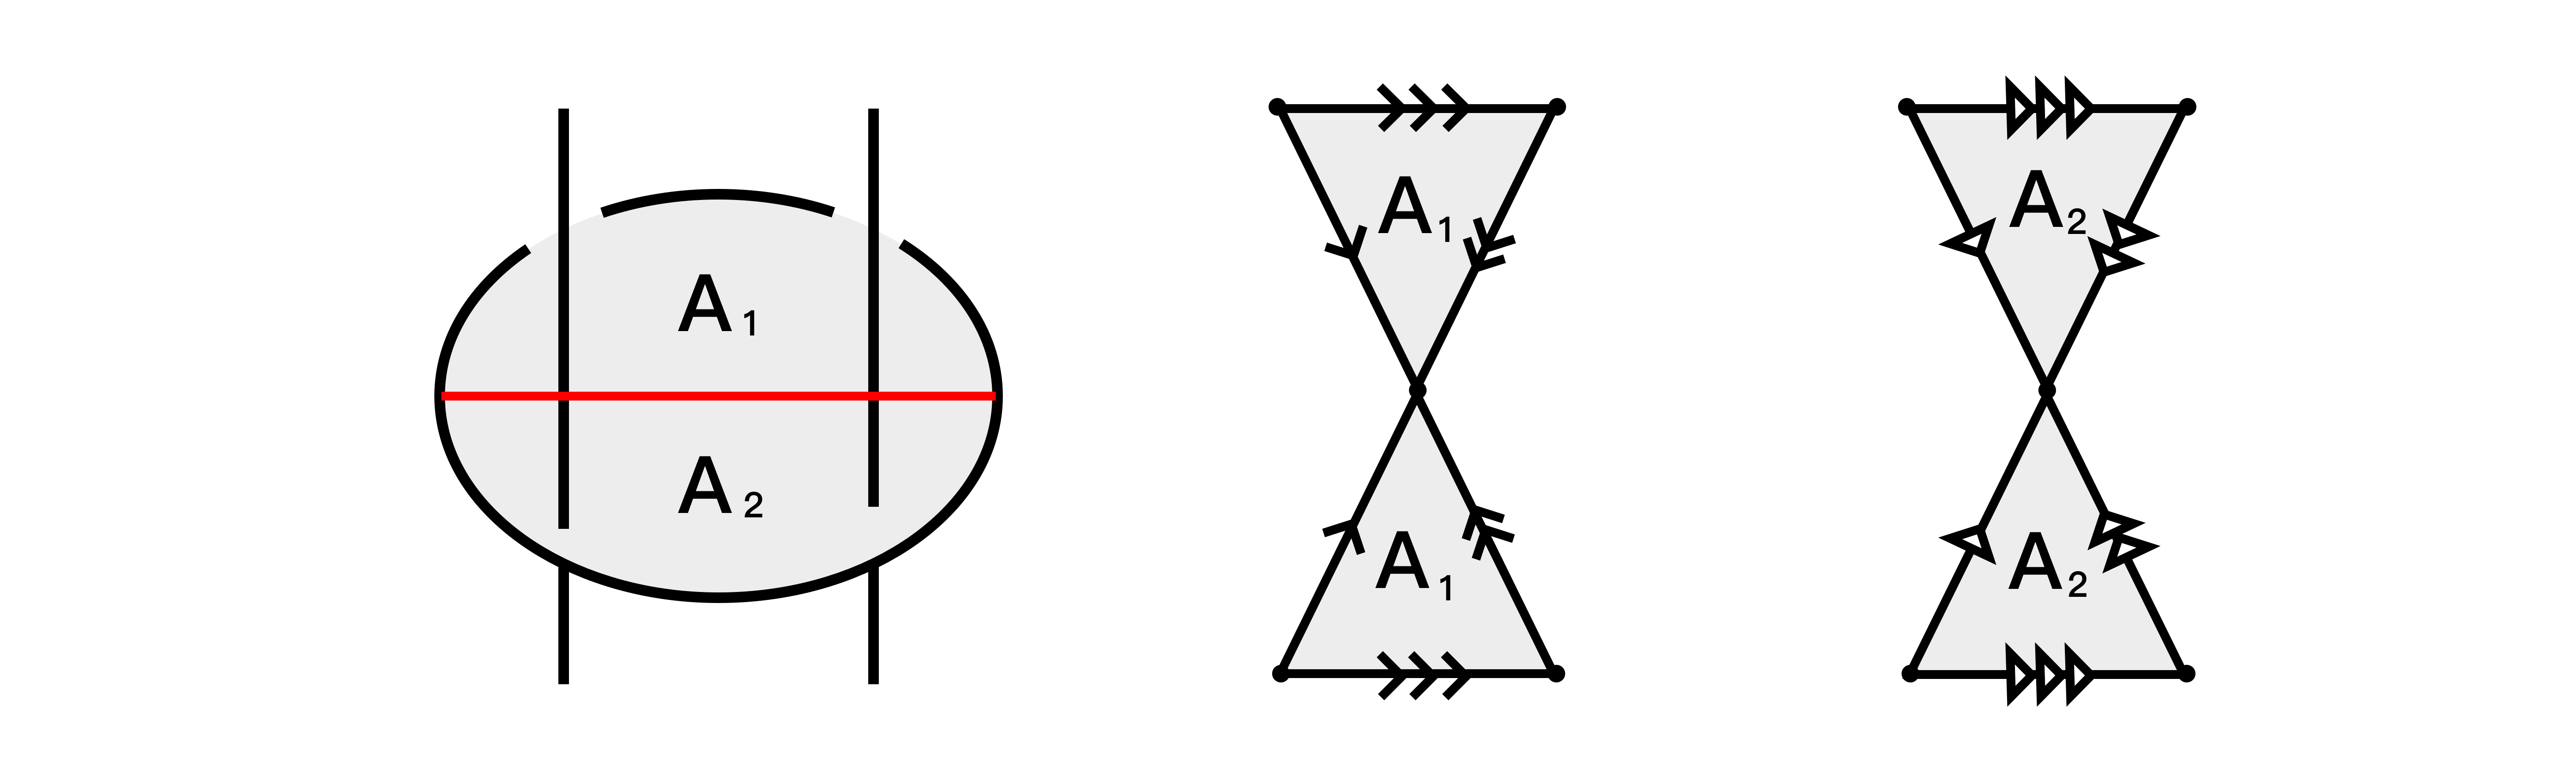
\includegraphics [width=8cm]{falGluing1.png}&
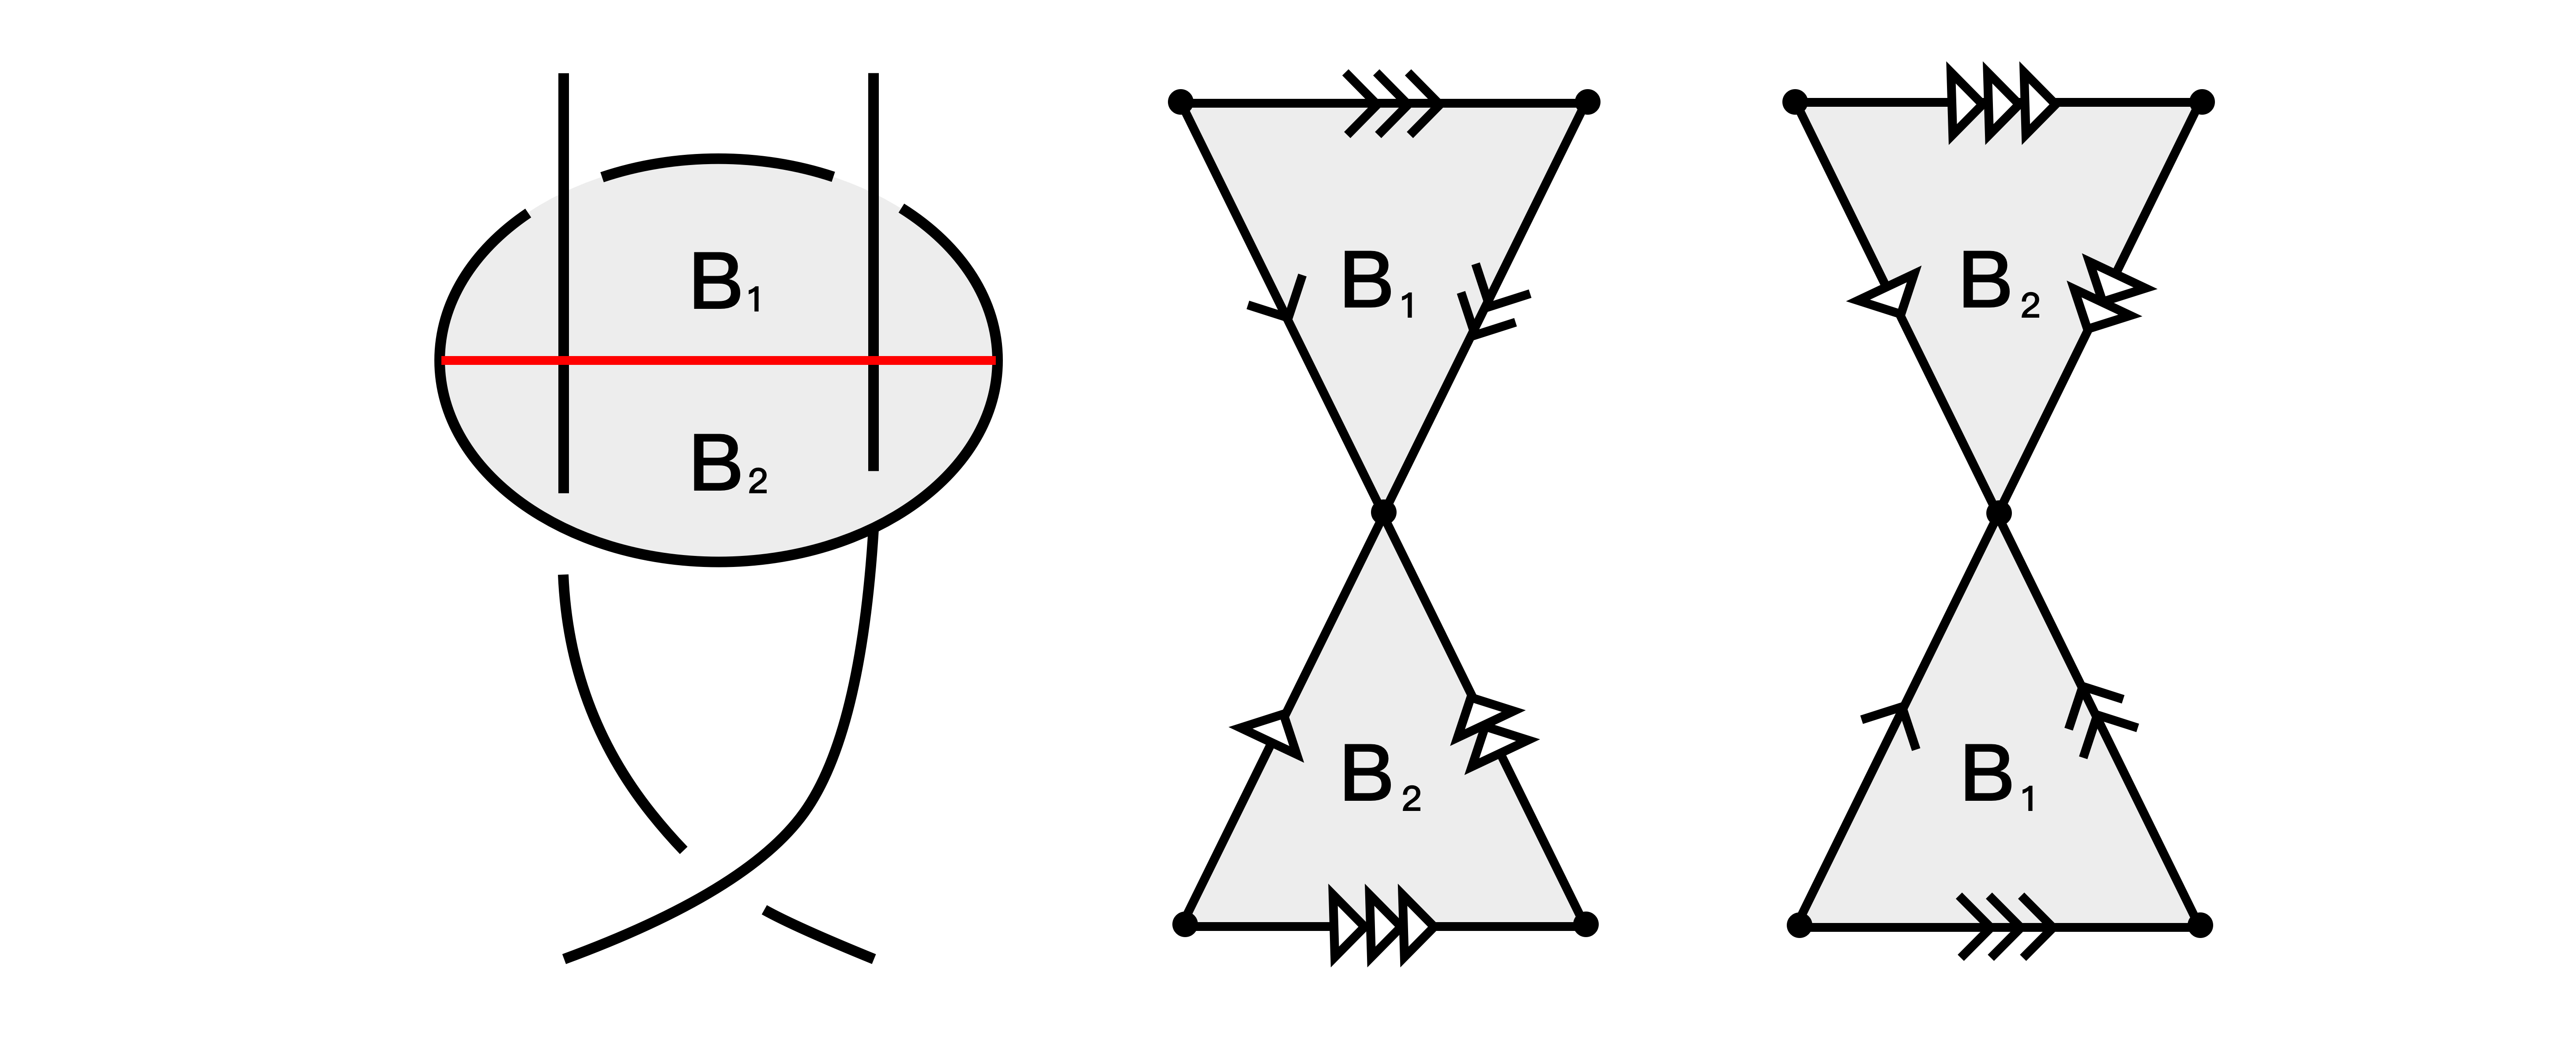
\includegraphics [width=7cm]{falGluing2.png}\\
(a)&(b)
\end{tabular}
\caption{(a) Gluing of bow-ties without half-twists
(b) Gluing with half-twists}
\label{fig:falGluings}
\end{figure}


The crossing edges and edges from spanning disks of crossing circles
form the graph of the top ideal torihedron.
We repeat the steps for the bottom half of $\torus \times I$, $\torus \times
(-1,0]$. Thus we get two ideal torihedra.
%The graph of each will come from
%crossing edges and edges from spanning disks of crossing circles.


We obtain the complement of $L$ by gluing the two torihedra with the gluing
information given by identifying crossing edges and triangles of the bow-tie. We
glue the faces of the torihedra which do not correspond to a bow-tie with a
$2\pi/n$ twist where $n$ is the number of sides of each face as in Figure
\ref{fig:top-bottom} clockwise or counterclockwise.


Now, if $L$ has half-twists,
we apply the constructions above to $L'$,
which is the link obtained from $L$ by removing all half-twists
(replacing them with parallel strands).
The complement of $L$ is again obtained by
gluing the torihedra together all the same,
except that at the bow-ties coming from twist regions with a half-twist,
they are glued as in Figure \ref{fig:falGluings} (b).
%we decompose the complement of the link the same way
%(as if there are no half twists)
%but we identify the two bow-ties as in Figure \ref{fig:falGluings} (b).
%Finally,


For future reference, we will denote the graph for the top and bottom
torihedra by $\Gamma_T(L)$ and $\Gamma_B(L)$, respectively,
where both graphs are viewed from the cone point of the top torihedron
$\torus \times \{1\}$.
Note that if $L = K$ is the non-augmented link,
$\Gamma_T(L)$ is simply the link projection of $K$,
and in fact $\Gamma_T(K) = \Gamma_B(K)$.


As promised, we give a description of (the graphs of) the torihedra
in terms of link diagrams of $K$ and $L$.
Let $D = D(K)$ be the link diagram of $K$,
and let $D'$ be the graph obtained from $D$
by collapsing each augmented twist region of $K$ to a vertex.
It is clear that $D'$ is the link diagram of a link $K'$
obtained from $K$ by removing half-twists from each augmented twist region
until one crossing remains.
Let $v_t$ denote a vertex of $D'$ corresponding to
an augmented twist region of $K$,
and let $v_c$ denote a vertex of $D'$ corresponding to
a crossing of $K$ not in an augmented twist region.


Orient the edges of $D'$ to point from an undercrossing
to an overcrossing.
Label the two outgoing edges at vertex $v$
(which corresponds to a crossing or a twist region)
by $e_v^{(1)}, e_v^{(2)}$ (in arbitrary order).
For each left- (resp. right-) augmented twist region $t$,
we perform a left (resp. right) bow-tie modification to
$v_t, e_{v_t}^{(1)}, e_{v_t}^{(2)}$.


The resulting graph is the graph $\Gamma_T(L)$
of the top torihedron.
If we had oriented the edges of $D'$ the other way,
and subsequently performed the same operations,
we would obtain $\Gamma_B(L)$ the graph of the bottom torihedron.


The non-bow-tie faces of $\Gamma_T(L)$ and $\Gamma_B(L)$
naturally correspond
(as the bow-tie modification procedure does not remove faces)
and are glued together.
\end{proof}



%%%%%%%%%%%%%%%%%%%%%%%%%%%%
The Figures \ref{fig:step_one} to \ref{fig:top-bottom}
depict an example which decomposes the link (C) of Figure
\ref{fig:Augmentations}. 


\begin{figure}[h] 
\centering
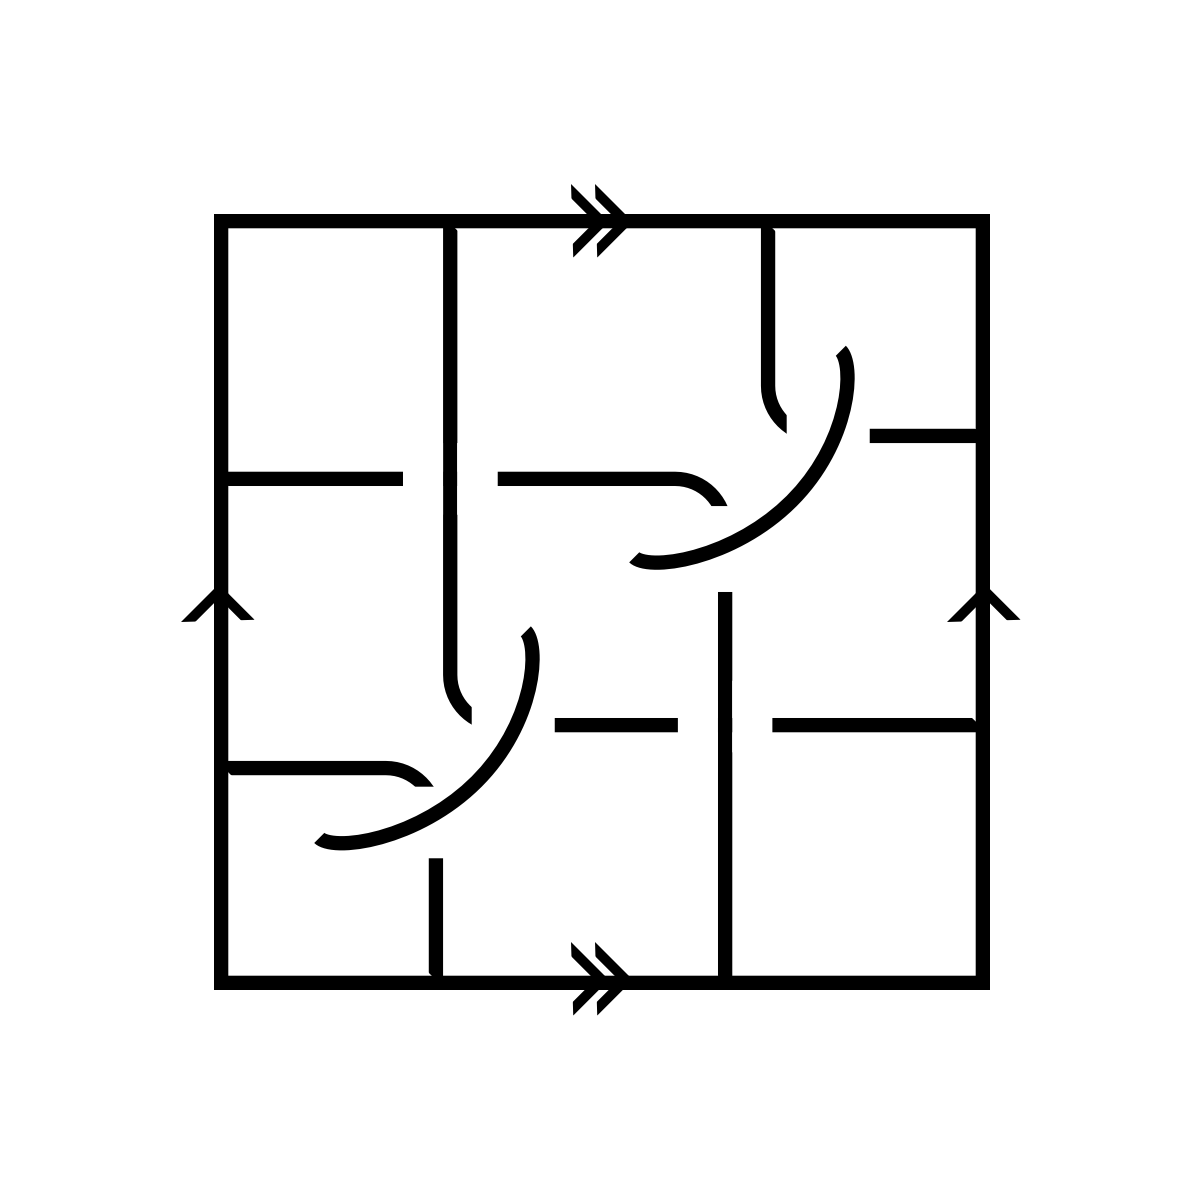
\includegraphics[height=3cm]{fig-3.png}
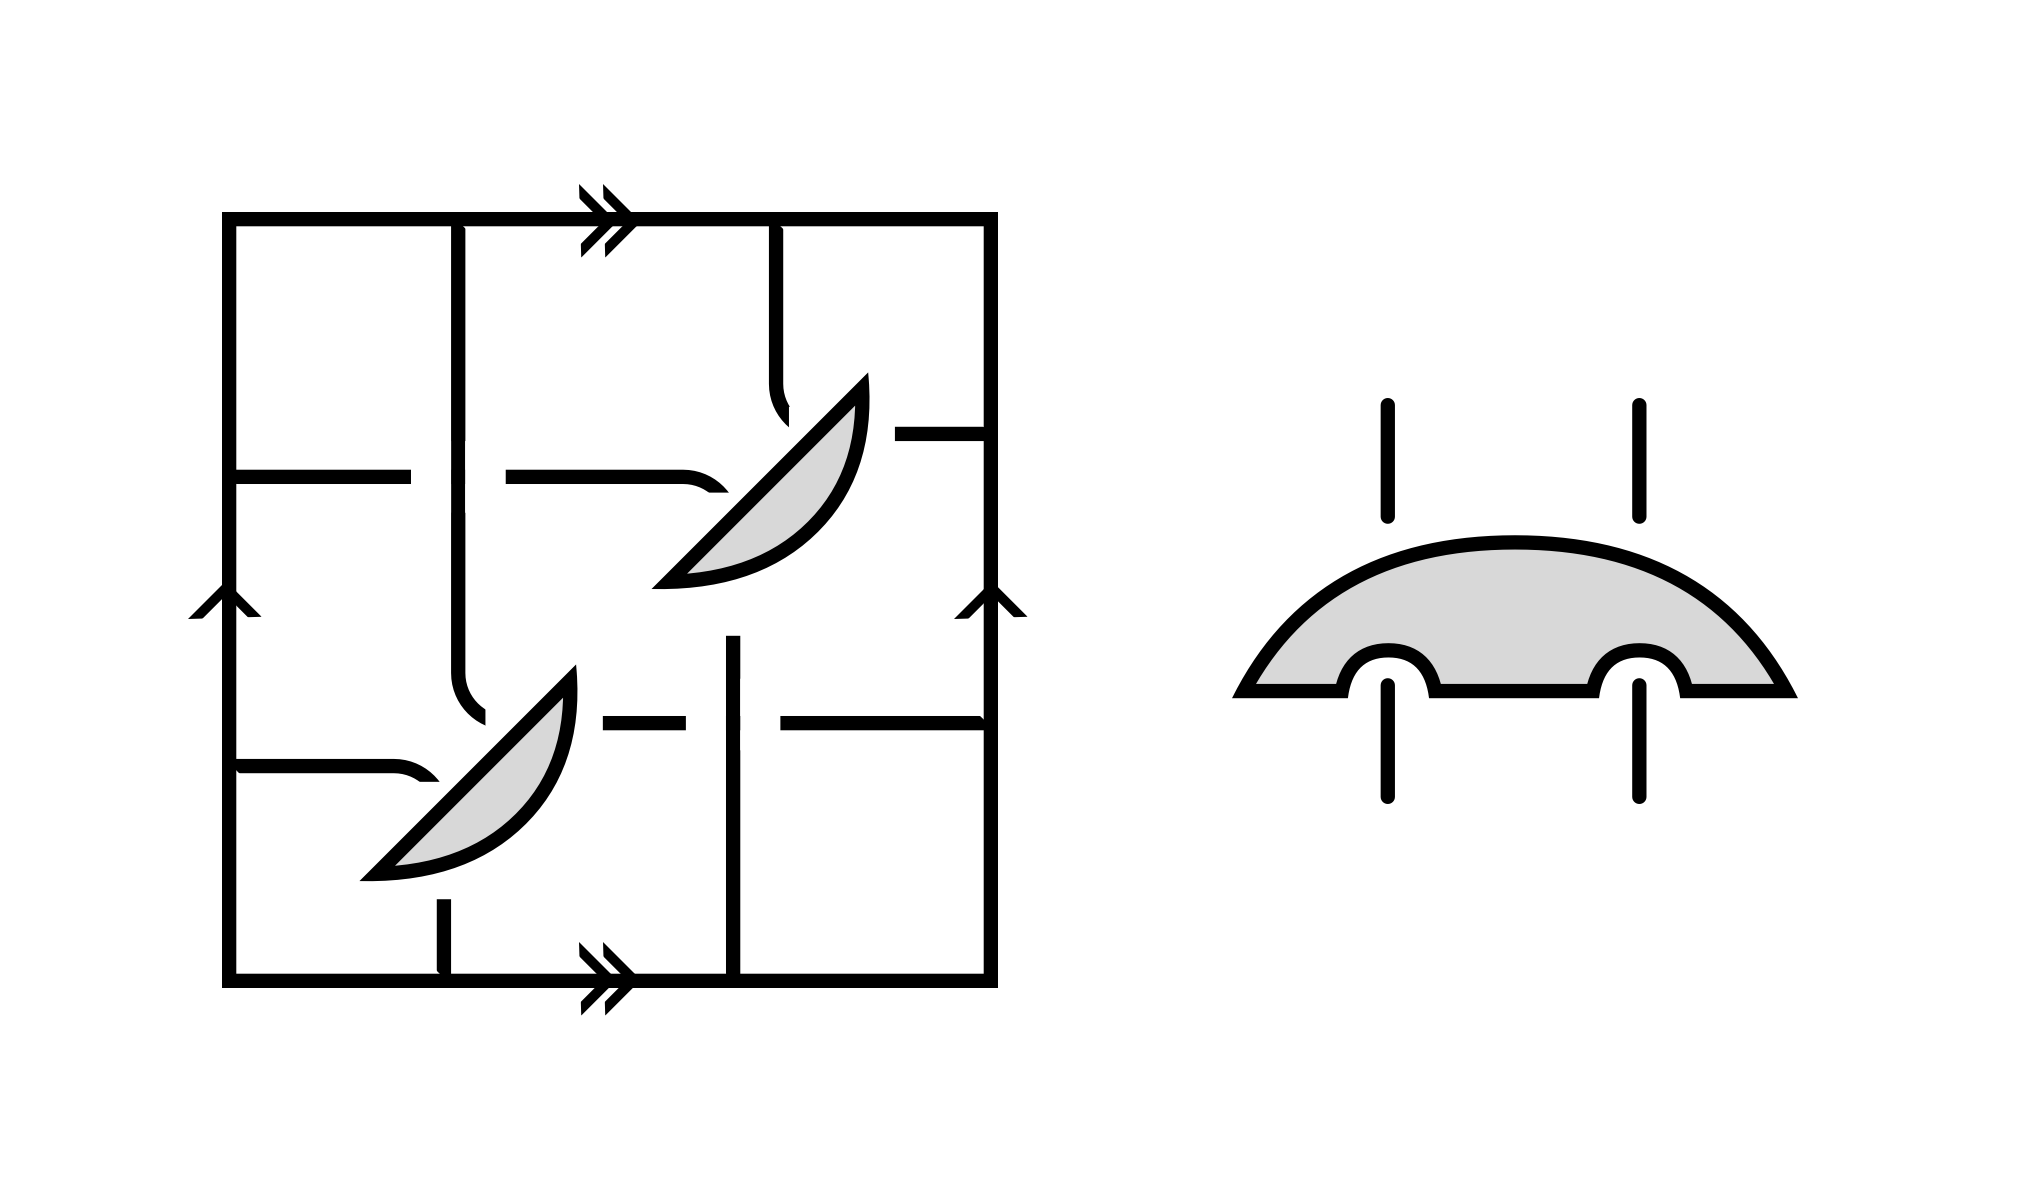
\includegraphics[height=3cm]{fig-4.png}
	\caption{Each crossing circle bounds a twice-punctured disk}
	\label{fig:step_one}
\end{figure}
 
%\vspace{-0.5cm} 
\begin{figure}[h] 
\centering 
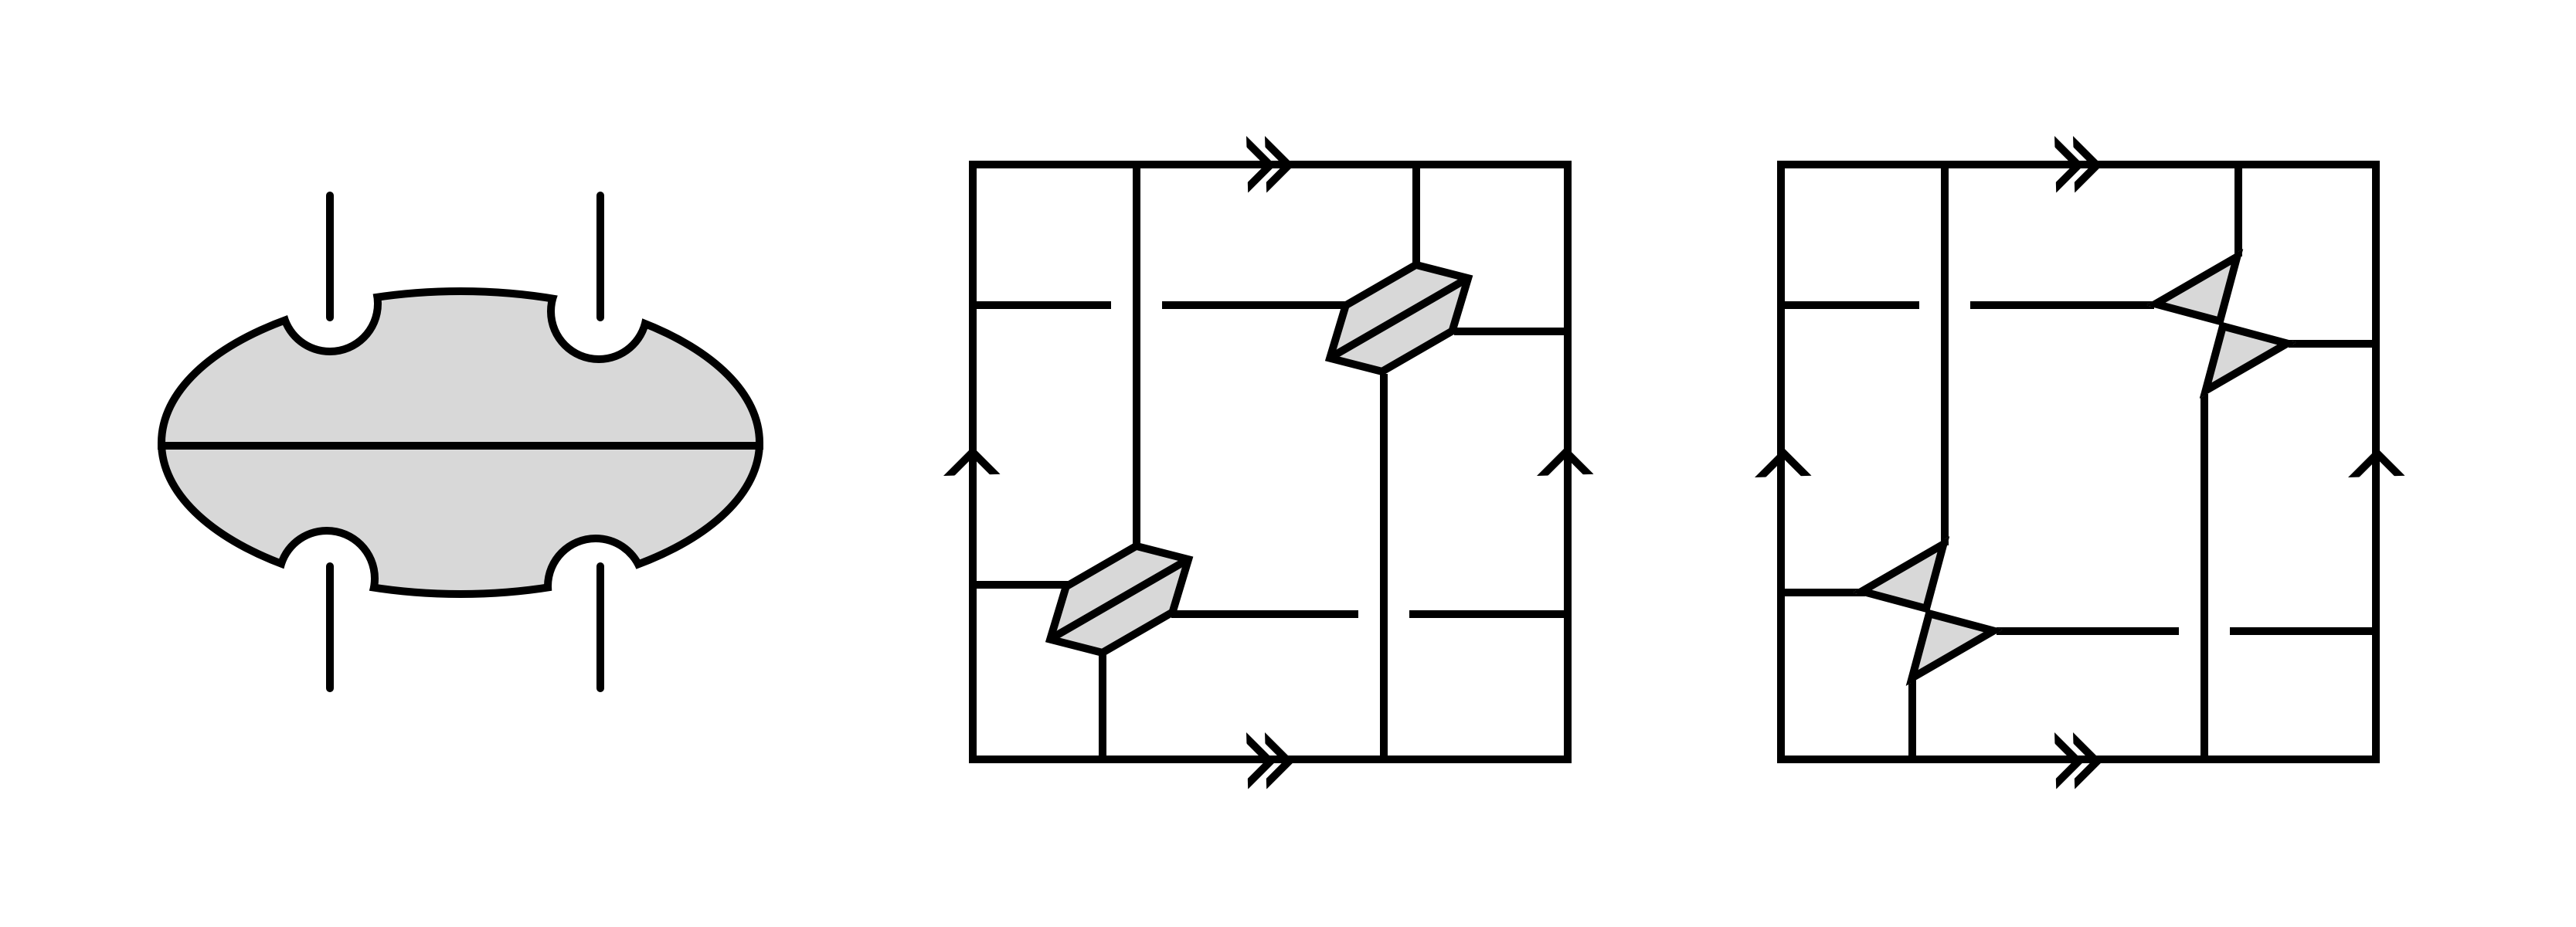
\includegraphics[height=3cm]{fig-5.png} 
	\caption{We split the disk and collapse the arc of each
 crossing circle to ideal vertices}
	\label{fig:step_two}
\end{figure}


\begin{figure}[h] 
\centering 
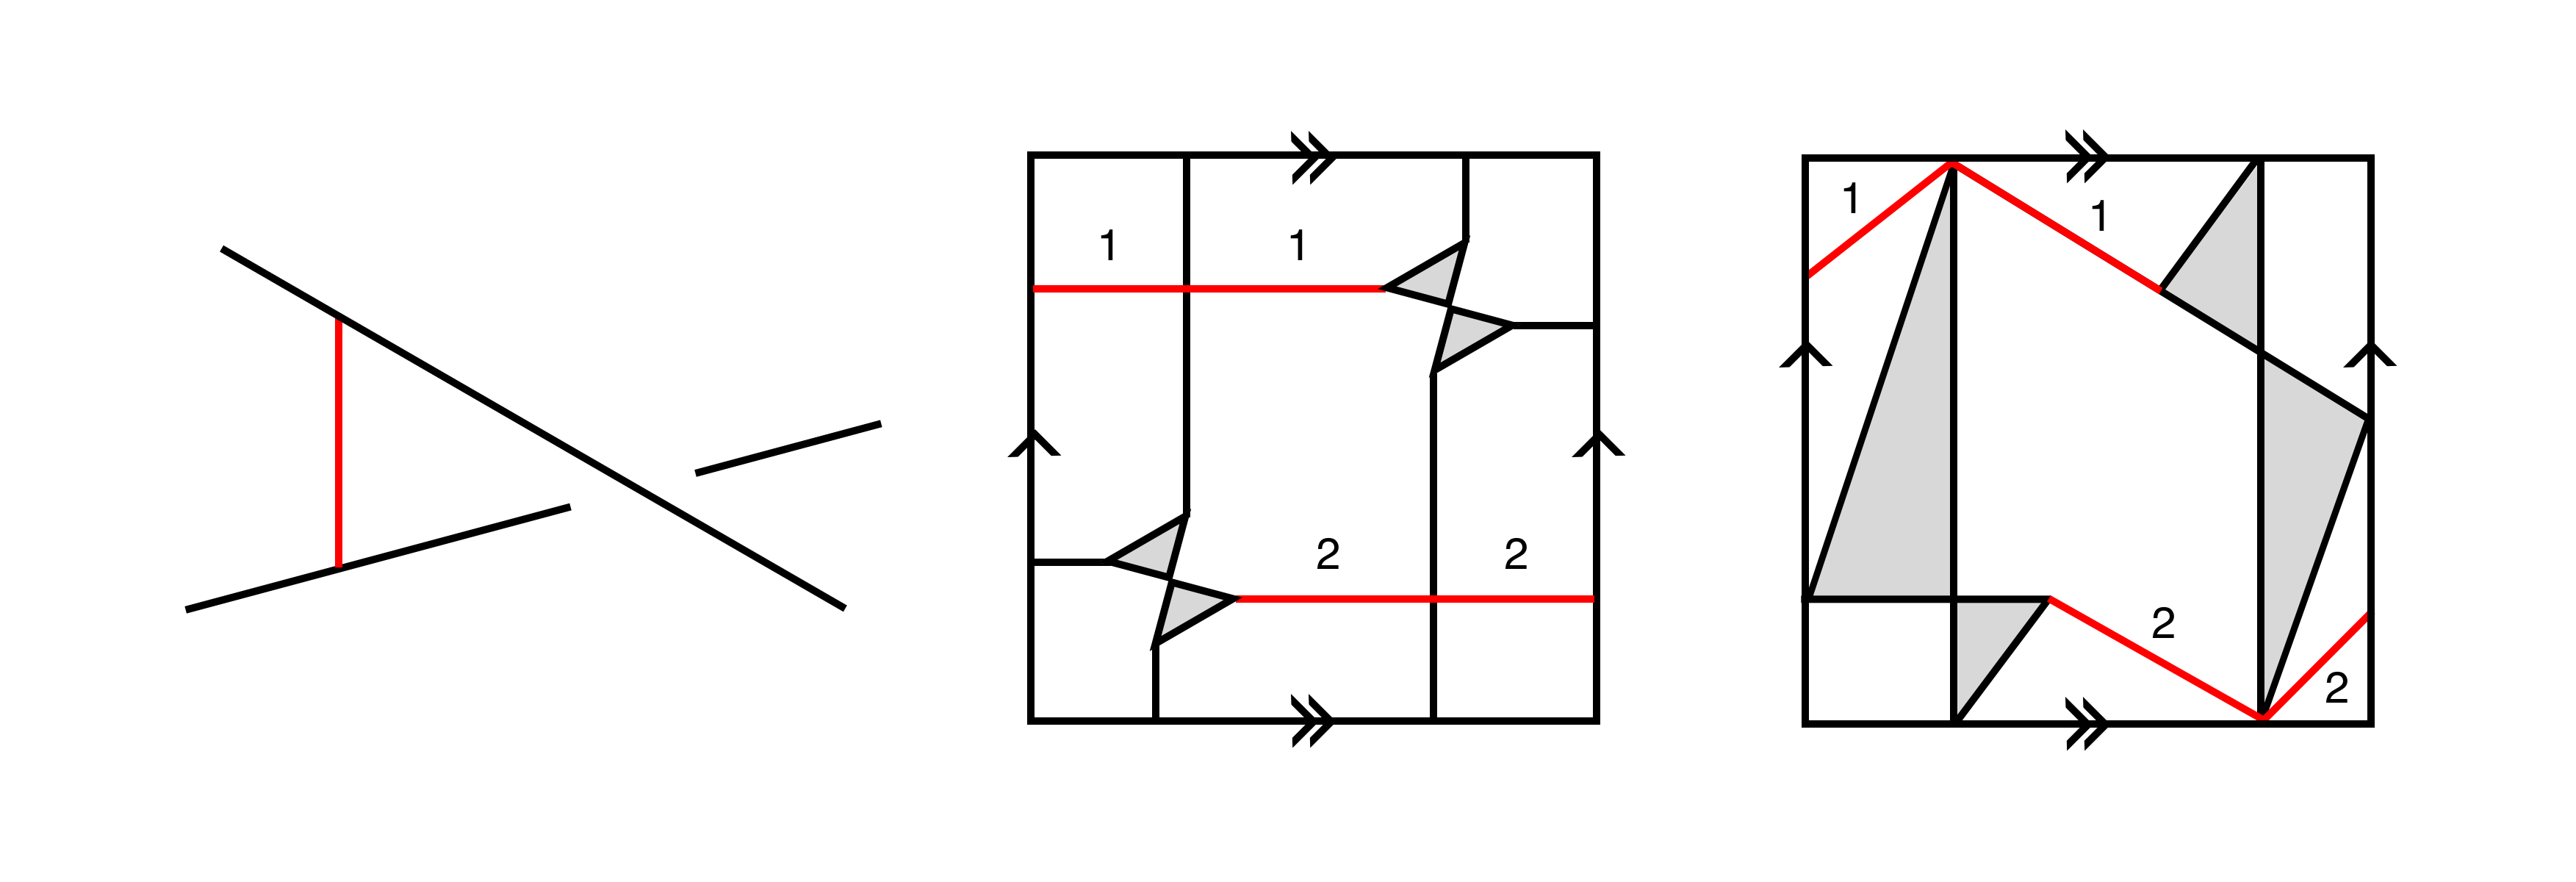
\includegraphics[height=3cm]{fig-6.png} 
\caption{Left: The crossing arc is the edge in red.
Middle: Picture of splitting the crossing edge.
Right: The link components are pushed off to infinity.}
	\label{fig:step_three}
\end{figure}

\begin{figure}[h] 
\centering 
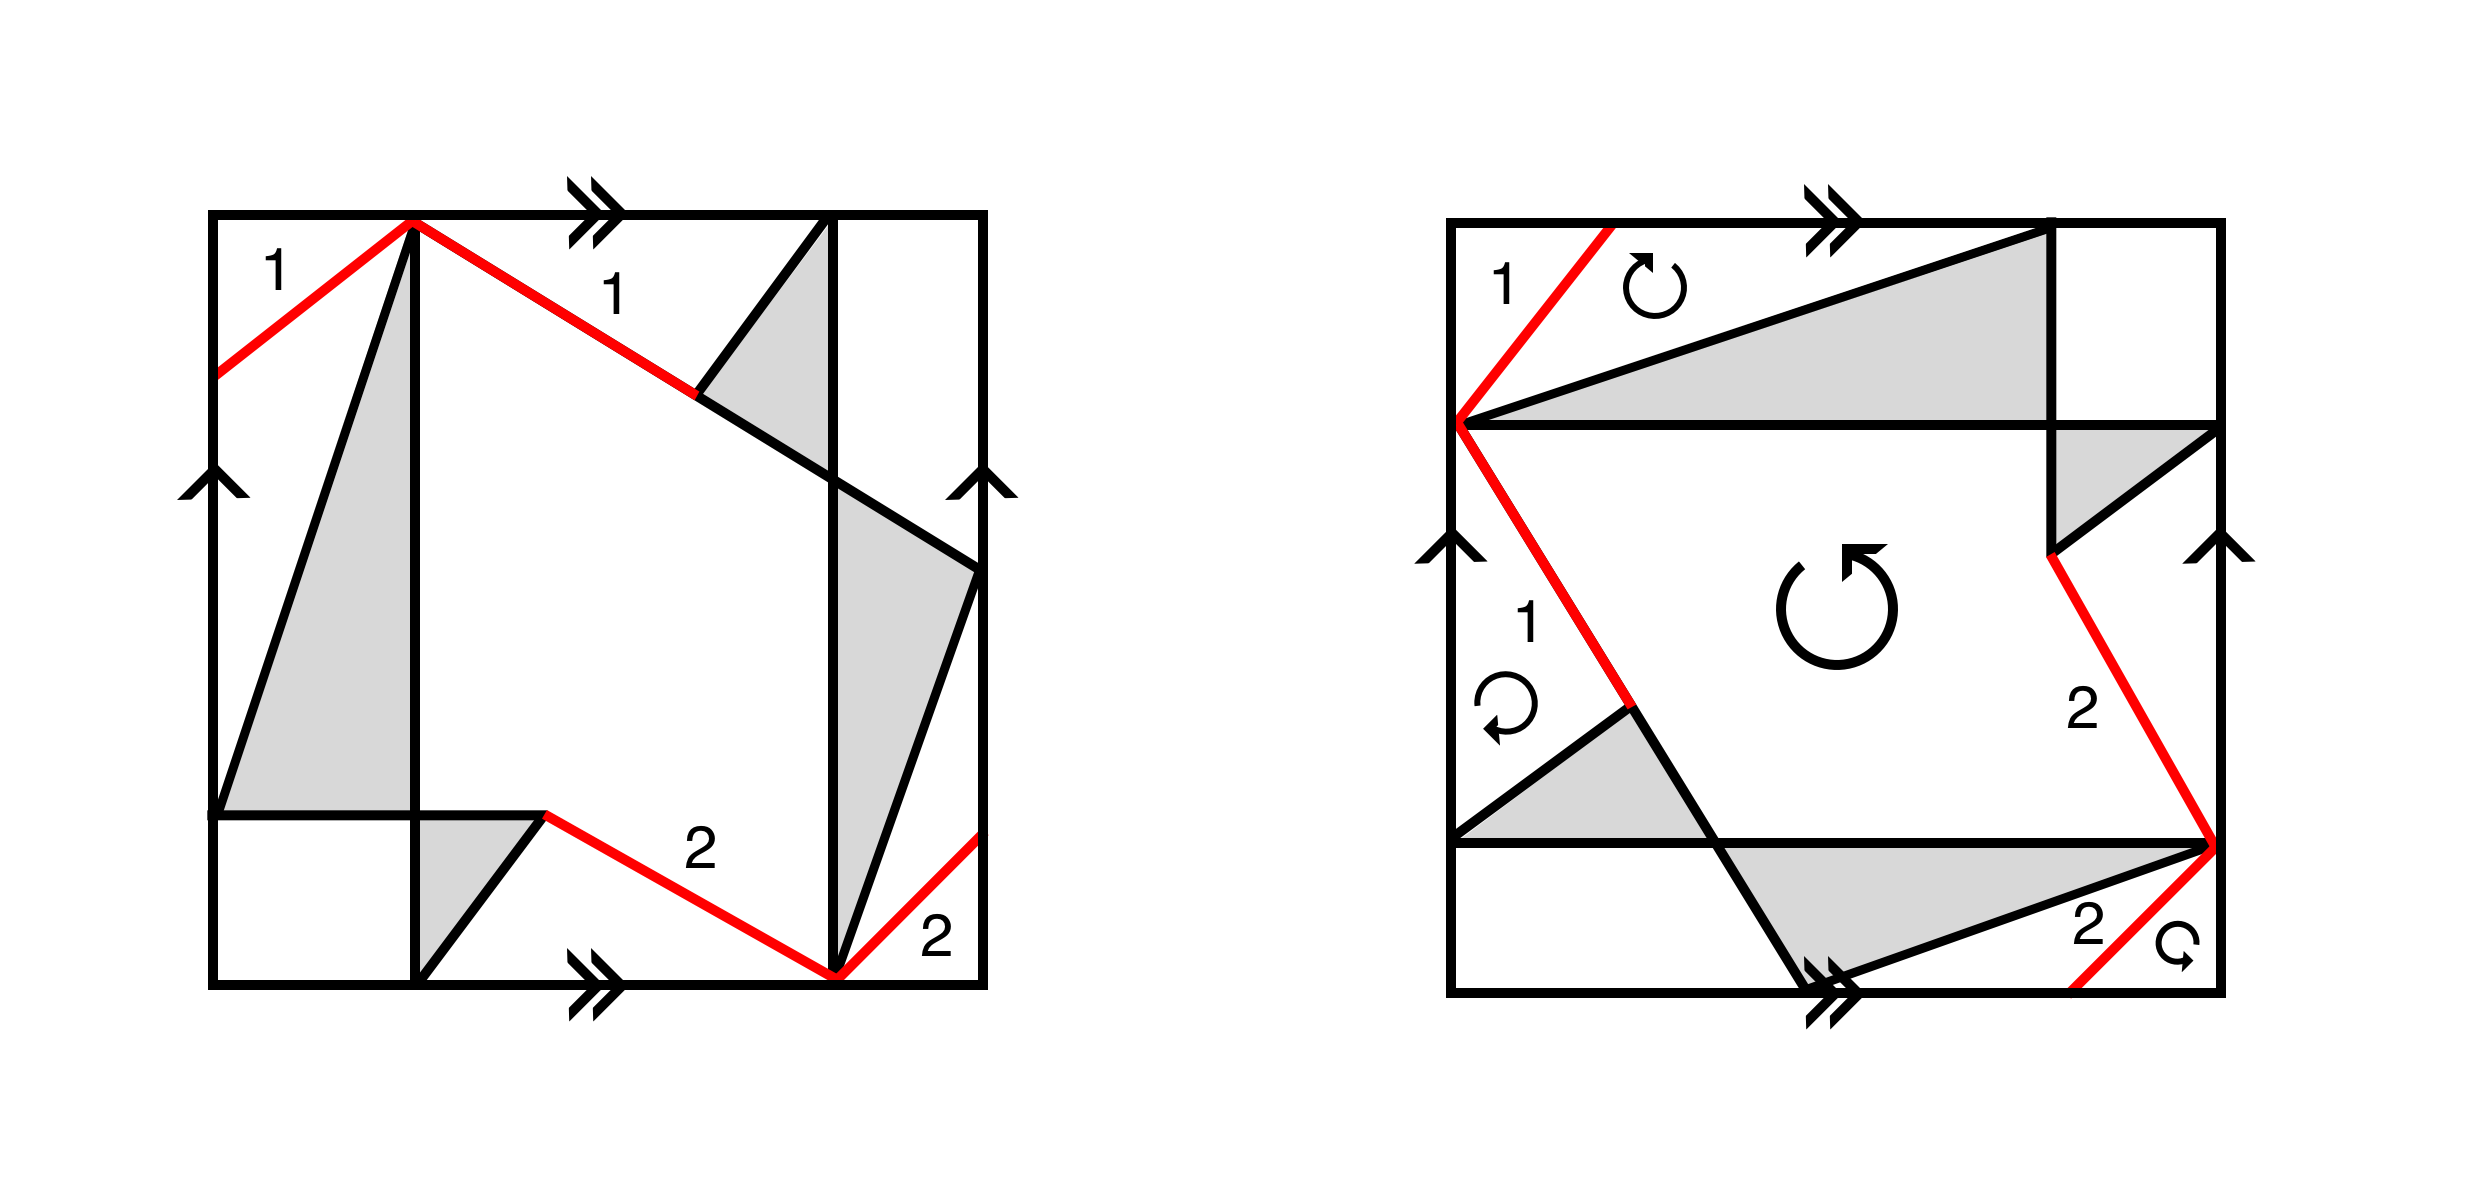
\includegraphics[height=3cm]{top-bottom.png} 
	\caption{Left: The top torihedron.
	Right: The bottom torihdron with rotation indicating face gluing;
	TODO shouldn't it be rotating other way?} 
\label{fig:top-bottom}
\end{figure}



\begin{definition}
An \emph{angled torihedron} $(\sT, \theta_\bullet^*)$
is a torihedron $\sT$ with
an assignment of an \emph{interior dihedral angle}
$\theta_e^* \in [0,\pi]$ to each edge $e$ of $G(\sT)$
such that for each vertex $v \in G(\sT)$,
$\sum_{e \ni v} \theta_e^* = (\deg(v) - 2)\pi$.
We also denote $\theta_e = \pi - \theta_e^*$,
so $\sum_{e \ni v} \theta_e = 2\pi$;
we refer to $\theta_e$ as the \emph{exterior dihedral angle}.
%and $\theta_e^*$ as the interior angle. 
For brevity, we write dihedral angle to mean 
interior dihedral angle.  


We say $(\sT, \theta_\bullet^*)$ is \emph{degenerate}
if $\theta_e^* = 0$ for some edge;
we say it is \emph{non-degenerate} otherwise.
\end{definition}


One may ask for the pyramidal decomposition of a torihedron
to ``respect" angles. The following definitions,
in particular an ``angle splitting'', make sense of this.

\begin{define}
An \emph{angled ideal tetrahedron} is an ideal tetrahedron
with an assignment of an
interior dihedral angle $\theta_e^*$ to each edge $e$, such that
\begin{itemize}
\item each dihedral angle is in $[0, \pi]$;
\item for each tetrahedron, opposite edges have equal dihedral angles;
\item the three distinct interior angles at edges incident to one vertex sum to $\pi$.
\end{itemize}

We say an angled ideal tetrahedron is \emph{degenerate} if
one dihedral angle is 0; we say it is \emph{non-degenerate} otherwise.
\end{define}


\begin{define}
A \emph{base-angled ideal pyramid}
is a pyramid whose base is an $n$-gon, $n \geq 3$,
and each boundary edge $e_i$ of the base face is assigned a dihedral angle
$\alpha_i \geq 0$ such that their sum is $\sum \alpha_i = \pi$.
The vertical edge $e_i'$ that meets $e_i$ and $e_{i+1}$
is automatically assigned the dihedral angle $\pi - \alpha_i - \alpha_{i+1}$.


We say a base-angled ideal pyramid is \emph{degenerate} if
$\alpha_i = 0$ for some $i$; we say it is \emph{non-degenerate} otherwise.
\end{define}


Clearly, the dihedral angles of an ideal hyperbolic pyramid
make it a base-angled ideal pyramid
(with $\alpha_i = \vphi_{e_i}$);
it is not hard to see that the converse is true:
simply consider a circumsribed polygon such that the side $e_i$
subtends an angle of $2\alpha_i$ at the center,
and take the ideal hyperbolic pyramid over it in upper-half space.
Also, an angled ideal tetrahedron is simply a base-angled ideal pyramid
with base a triangle, and with no preferred face.

\begin{definition}
%TODO: this definition should come after base-angled pyramid
An \emph{angle splitting} of an angled torihedron $(\sT,\theta_\bullet^*)$
is an assignment of an angle $\vphi_{\vec{e}}$ to each
oriented edge $\vec{e}$, such that

\begin{itemize}
\item for each edge $e$,
$\theta_e^* = \vphi_{\vec{e}} + \vphi_{\cev{e}}$,
where $\cev{e}$ is the opposite orientation on $e$,
\item for each face $f$,
$\sum_{\vec{e} \in \del f} \vphi_{\vec{e}} = \pi$,
where $\vec{e} \in \del f$ is the edge in the boundary of $f$
taken with outward orientation.
\end{itemize}


Equivalently, an angle splitting is a decomposition of
$\sT$ into base-angled pyramids,
one for each face of $G(\sT)$, such that
for each boundary edge $e$ of $\sT$,
the dihedral angles from the two adjacent pyramids
add to $\theta_e^*$.


We also say that $\vphi_\bullet$ is an angle-splitting
of the edge-labeled graph $(G(\sT), \theta_\bullet^*)$.


We say that an angle-splitting is \emph{degenerate}
if $\vphi_{\vec{e}} = 0$ for some oriented edge $\vec{e}$;
it is \emph{non-degenerate} otherwise.
\end{definition}

\begin{remark}
These $\theta$'s are the same as the $\theta$'s in
\cite{BandS},
and angle-splittings $\vphi_\bullet$'s
are the same as their ``coherent angle system''.
\end{remark}


%TODO remark on what splitting means in terms of ideal hyperbolic

\begin{lemma}
\label{l:pyramid_decomp}
%Let $P_n$ be an ideal pyramid whose base is an $n$-gon and suppose,
%\begin{itemize}
%\item each boundary edge of the base face is assigned a dihedral angle $\alpha_i$ such that for adjacent edges, $\alpha_i + \alpha_{i+1} < \pi$;
%\item we are given a decomposition of the base face into triangles by adding new edges. 
%\end{itemize}
Let $P_n$ be a base-angled ideal pyramid, and suppose we are given a
decomposition of the base face into triangles by adding new edges.  One gets an
obvious corresponding triangulation of $P_n$, where a new face is added for each
new edge. Then there is an assignment of a dihedral angle to each edge of each
ideal tetrahedron in this triangulation such that
\begin{itemize}
\item each tetrahedron is an angled ideal tetrahedron;
\item the sum of dihedral angles around each new edge is $\pi$;
\item the dihedral angles of the edges of the original base face are the same as
	before.
\end{itemize} 
Moreover, if $P_n$ is non-degenerate,
then the resulting angled tetrahedra are also non-degenerate.
\end{lemma}

\begin{proof}
Induct on $n$; there is nothing to prove for the base case $n=3$.


The proof is essentially given in Figure \ref{f:ideal_pyramid_arg}.
We spell it out here in words.


\begin{figure}
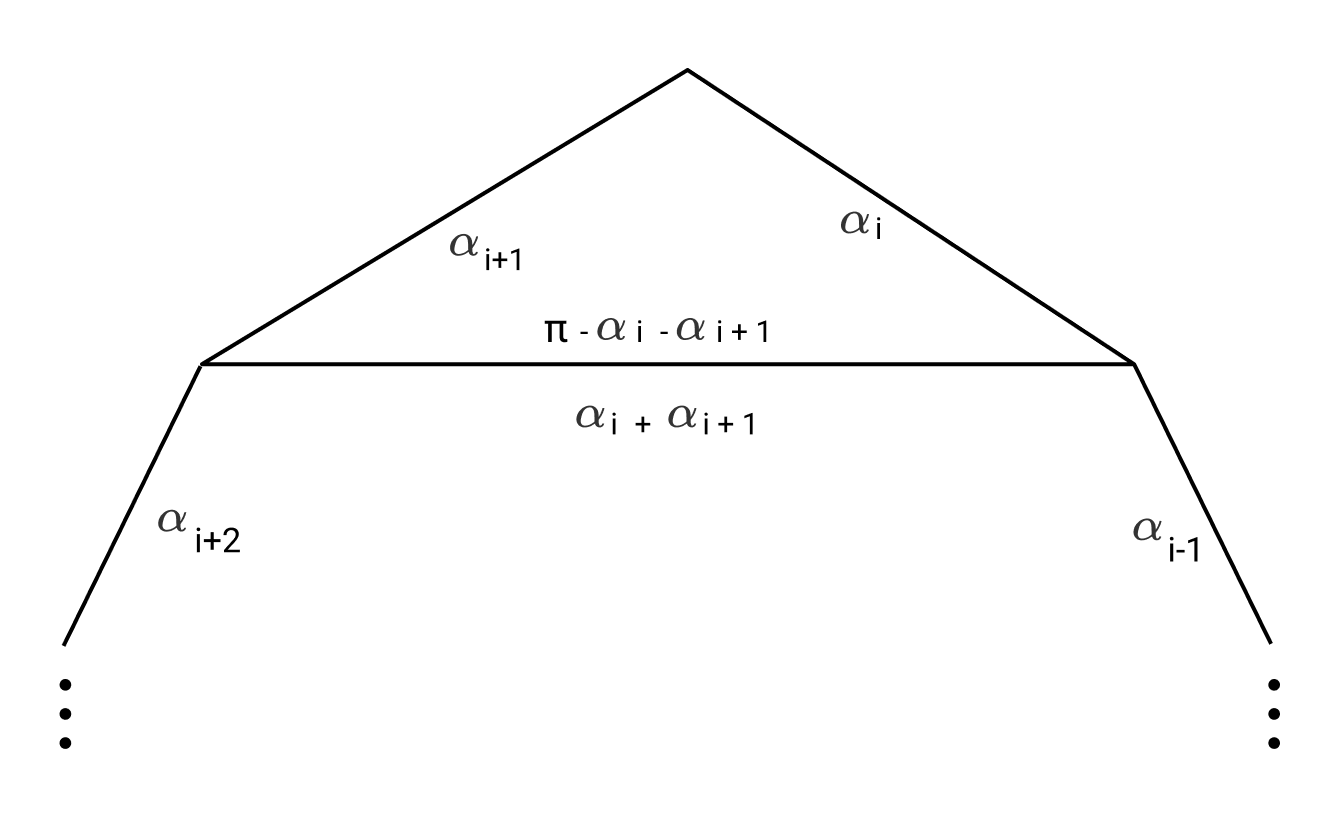
\includegraphics[height=5cm]{more_pictures/angle_split.png}
\caption{Angle-splitting on a polygonal face of the graph}
\label{f:ideal_pyramid_arg}
\end{figure}


Suppose the edges are labeled $e_i$, for an edge
which goes between vertices $v_i$ and $v_{i+1}$,
and suppose $e_i$ is assigned dihedral angle $\alpha_i$.
Let $e'$ be a new edge addeed to the base face of $P_n$
such that it separates the base face into a triangle and
an $(n-1)$-gon;
suppose the sides of the triangle are
$e_i, e_{i+1}$, and $e'$.
The new face corresponding to $e'$ separates $P_n$ into
an ideal tetrahedron $T$ and an ideal pyramid $P_{n-1}$.
We assign the dihedral angle of $\pi - \alpha_i - \alpha_{i+1}$
to $e'$ in $T$, and assign $\alpha_i + \alpha_{i+1}$ to $e'$ in $P_{n-1}$.
Clearly the sum of dihedral angles condition is satisfied
in $T$ and $P_{n-1}$.
It remains to check that the dihedral angles assigned to the vertical (non-base)
edges are correct.
For the vertical edge associated to $v_j$ for $j \neq i, i+2$,
there is nothing to check;
for $j = i$, the dihedral angles are
$\pi - \alpha_i - (\pi - \alpha_i - \alpha_{i-1})$
in $T$ and $\pi - \alpha_{i-1} - (\alpha_i + \alpha_{i+1})$ in $P_{n-1}$,
which sum to $\pi - \alpha_i - \alpha_{i+1}$;
it is similar for $j = i+2$.


Non-degeneracy of the resulting angled tetrahedra
follows easily from the observation that the angles
assigned to each side of a new edge is simply the sum
of the angles of original edges on the other side.
\end{proof}


%%%%%%%%%%%%%%%%%%%%%%%%%%%%%%%%%%%%%%%%%%%%%%%%%%%%%%%%%%%
\section{Hyperbolicity of Augmented Links}
\label{s:hyperbolicity}
Thurston introduced a method for finding the
unique complete hyperbolic metric for a given 3-manifold $M$
with boundary consisting of tori \cite{Thurston}. 
%The idea
%was to triangulate the interior of $M$ into ideal tetrahedra and give those
%tetrahedra hyperbolic shapes (called shape parameters) that glue up coherently
%in $M$. The shape parameter of a tetrahedron is described by the cross-ratio of
%its four vertices on the sphere at infinity. 
Thurston wrote down a system of gluing and consistency equations
which can be translated to equations involving
angles for a triangulation of $M$ whose solutions correspond to the
complete hyperbolic metric on the interior of $M$.
Casson and Rivin separated Thurston's
gluing equations into a linear and non-linear part \cite{Casson-Rivin}.
Angle structures are solutions to the linear part of
Thurston's gluing equations;
we will use them to attain hyperbolicity of complements
of augmented links in the thickened torus.


\begin{define}
Let $M$ be an orientable 3-manifold with boundary consisting of tori. An angle
structure on an ideal triangulation $\tau$ of $M$ is an assignment of a dihedral
angle to each edge of each tetrahedron, such that
\begin{itemize}
\item each tetrahedron is a non-degenerate angled ideal tetrahedron,
\item around each edge of $\tau$, the dihedral angles sum to $2\pi$.
\end{itemize}
\end{define}

%\cite{TODO: find rivin's paper? should be in here https://arxiv.org/pdf/1004.0440.pdf}


\begin{theorem}\cite[Theorem 1.1]{FG-angles}
Let $M$ be a 3-manifold with a triangulation that admits an angle structure.
Then $M$ is hyperbolic.
\end{theorem}


For a hyperbolic link $K$ in $\torus \times I$, we show
that the link $L$ obtained from augmenting $K$ is hyperbolic.
The idea is to start with a graph from the torihedral decomposition
of the link $K$ which will give us a graph on each torihedron with an angle
assignment of $\pi/2$ to each edge \cite{CKP2}.
By \prpref{p:tori_decomp},
there is a torihedral decomposition of the complement of the augmented link $L$.
Using those angles from $K$,
we then assign new angles locally to edges of torihedra from a torihedral 
decomposition of $L$
and decompose them into base-angled pyramids which can be decomposed 
into tetrahedra, thus obtaining an angle structure on a triangulation.




We need the following theorem,
adapted from \cite[Theorem 4]{BandS},
specialized to genus 1 surfaces:


\begin{theorem}{\cite[Theorem 4]{BandS}}
Let $\Gamma = (V,E)$ be a graph on the torus,
and let $\Gamma^* = (F,E^*)$ be the dual graph,
with $E^*$ being naturally identified with $E$.
Let $\theta_\bullet \in (0,\pi)^E$
be a function on the set of edges $E$
that sums to $2\pi$ around each vertex of $V$.


There exists an angle-splitting of $(\Gamma,\theta_\bullet)$
if and only if the following
``cocycle condition'' is satisfied:

\begin{quotation}
Suppose we cut the torus along a subset of edges in the dual graph
$\Gamma^*$, obtaining one or more pieces;
Then for any piece that is a disc,
the sum of $\theta_\bullet$ over the edges in the boundary
of the piece is at least $2\pi$,
with equality if and only if the piece
contains exactly one vertex of $\Gamma$.
\end{quotation}

\label{t:bs-thm4}
\end{theorem}

The original theorem \cite[Theorem 4]{BandS}
proves that a circle pattern combinatorially equivalent to $\Gamma$
exists; a circle pattern naturally yields
an angle-splitting (which they call a coherent angle system).


\begin{theorem}
\label{t:auglink_hyp}
Let $K$ be a weakly prime, alternating link
in the thickened torus
whose diagram is cellular and has no bigons.
Let $L$ be a link obtained from augmenting $K$.
Then $L$ is hyperbolic.


More generally, if $K$ is as above with a twist-reduced diagram
containing bigons,
and $L$ is obtained by augmenting $K$
at every twist region with at least one bigon
(and possibly other crossings),
then $L$ is hyperbolic.
\end{theorem}

\begin{proof}
Let us first consider the case when $K$ did not have bigons.


By \cite[Theorem 7.5]{CKP2},
(as discussed in \prpref{p:tori_decomp},)
$\toruscomp{K}$ can be decomposed
into two torihedra $\sT_T$ and $\sT_B$,
with $\sT_T$ meeting the top cone point $\torus \times \{1\}$
and $\sT_B$ meeting the bottom cone point $\torus \times \{-1\}$.
We denote their graphs by $\Gamma_T(K), \Gamma_B(K)$ respectively;
viewed from the top cone point $\torus \times \{1\}$,
both graphs are the same as the projection graph of $K$.
%which we denote by $\Gamma$.
We make them non-degenerate angled torihedra by assigning $\theta^* = \pi/2$
for all edges.
%%Unlike in the case of alternating links or fully augmented links 
%%in the thickened torus we cannot make all angles $\pi/2$. This is 
%%because in our decomposition the vertices of the graph which
%%defines our torihedra are not all four valent. 


Using the fact that $K$ is weakly prime,
it is not hard to see that the ``cocycle condition''
of \thmref{t:bs-thm4} is satisfied.


\begin{figure}
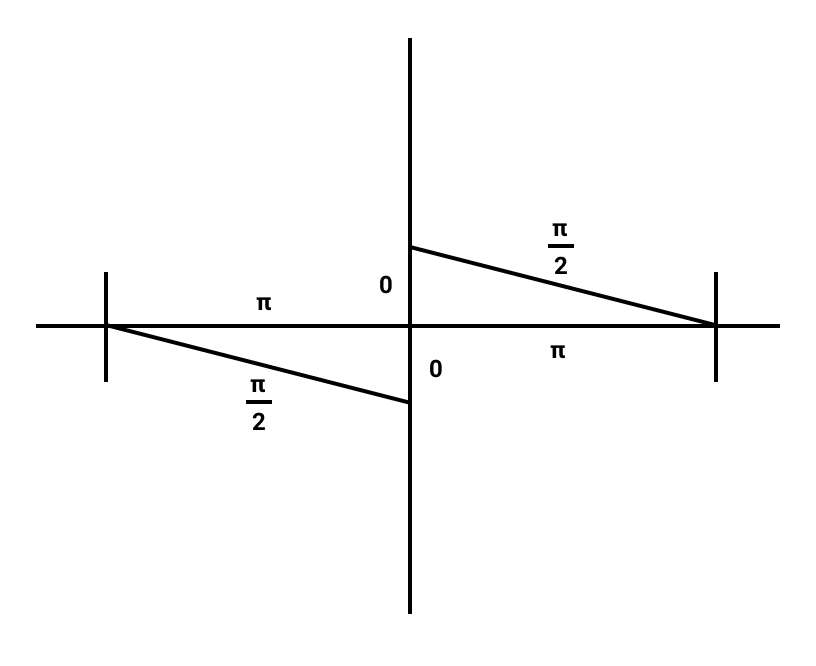
\includegraphics[width=7cm]{more_pictures/horizontal_bowtie.png}
\caption{Assignments of $\theta^*$ to edges of a bow-tie
	corresponding to an augmentation site}
\label{f:bowtie_angles}
\end{figure}

By \prpref{p:tori_decomp}, $\toruscomp{L}$ can be
obtained by gluing two torihedra $\sT_T(L),\sT_B(L)$
with graphs $\Gamma_T(L),\Gamma_B(L)$.
We make them degenerate angled torihedra by assigning $\theta^*$'s
to edges of the bow-ties as in Figure \ref{f:bowtie_angles},
and assign $\pi/2$ to all other edges.
It is easy to check that upon gluing,
each edge has sum of dihedral angles ($\theta^*$) that is equal to $2\pi$.
(This holds true even if they were glued assuming
some augmentations had no half-twist;
see end of proof where we deal with $K$ having bigons.)
%\remref{r:nohalftwist}.)


Furthermore, we can obtain an angle-splitting of $\sT_T(L)$
(and similarly $\sT_B(L)$) by modifying the angle-splitting
for $\sT_T(K)$;
this is shown in Figure \ref{f:bowtie_angles2}. 


\begin{figure}
\begin{tabular}{cc}
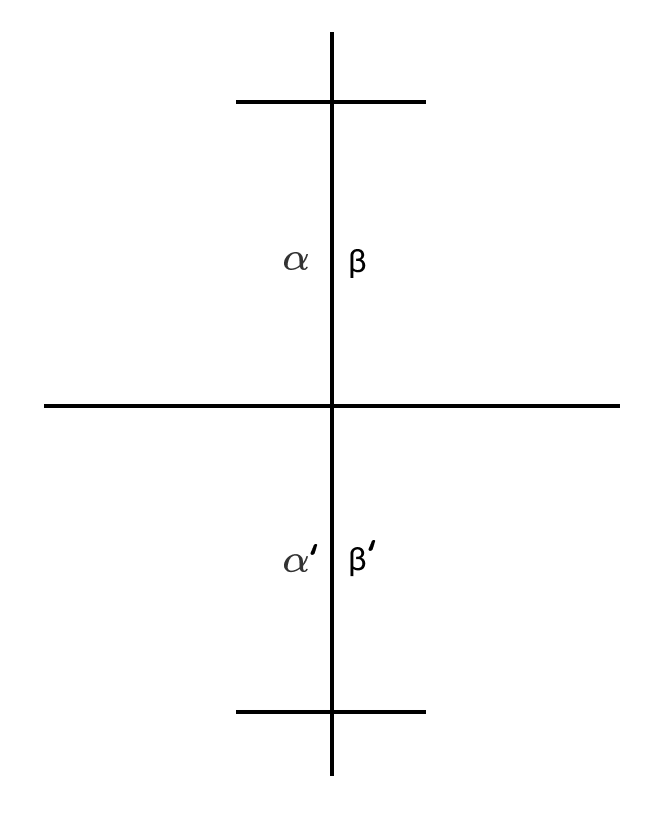
\includegraphics[width = 5cm]{before_bowtie_angles.png}&
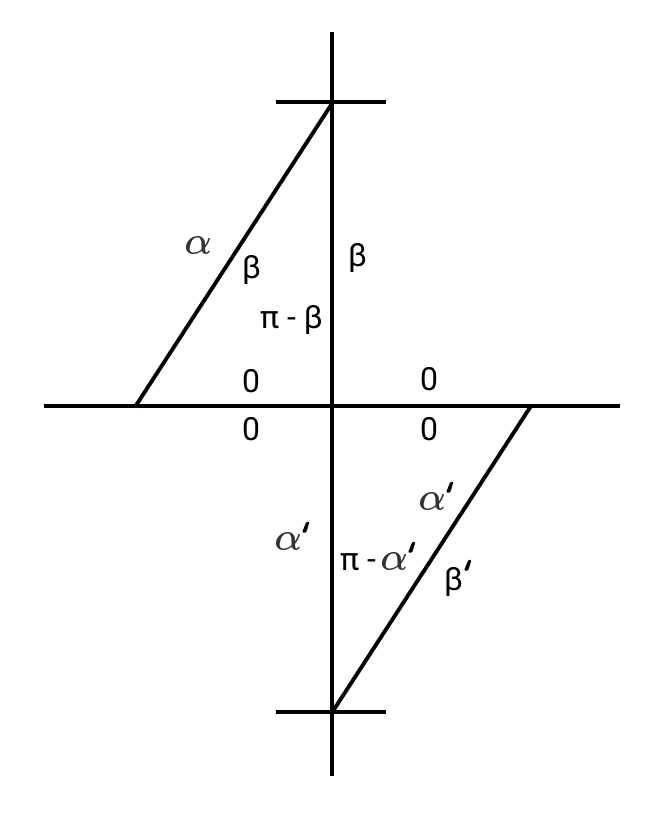
\includegraphics[width = 5cm]{bowtie_angles.png}\\
(a)&(b)
\end{tabular}
\caption{(a) Angle splitting before augmentation (b) Angle splitting for bowtie corresponding to augmentation}
\label{f:bowtie_angles2}
\end{figure}

Now we have a decomposition of the two torihedra into
degenerate base-angled pyramids.
However, we need the pyramids to be non-degenerate,
so we first need to modify the angles and graph on the torihedra
to make all $\theta^*$ nonzero.


Consider a face $f$ of $\Gamma_T(L)$ that is not in a bow-tie.
Suppose the corresponding face $\bar{f}$ of $\Gamma$,
the projection graph (which is equal to $\Gamma_T(K)$),
had vertices $v_1,\ldots,v_n$ in counter-clockwise order.
We label the edges of $f$ by $e_{i,0}$, $e_{i,\pi}$, or $e_i$,
depending on whether the $\theta^*$ is $0$, $\pi$, or $\pi/2$ respectively,
with $i$ non-decreasing from 1 to $n$,
adjacent edges having the same $i$ if and only if they
belong to the same bow-tie.
For sake of concreteness,
suppose that if a vertex $v_i$ is right-augmented,
then the augmentation circle intersects $\bar{f}$
(everything is similar if it is left-augmented vertices' circles
that intersect $\bar{f}$).
In other words, locally, $f$ meets two of the edges of the bow-tie
corresponding to a right-augmented vertex $v_i$
(which would be labeled $e_{i,0}, e_{i,\pi}$ in counter-clockwise order),
but only meets one of the edges of the bow-tie corresponding to
a left-augmented vertex.


Suppose, after cyclically reindexing, $v_1,\ldots,v_k$
is a maximally contiguous subsequence of left-augmented vertices
of $G(K)$ around the face $\bar{f}$;
the edges around $f$ would start
$e_{1,0}, e_{1,\pi}, e_{2,0}, e_{2,\pi}, \ldots$.
We add new edges across $f$ as follows.
(See Figure \ref{f:adding_edges};
ignore the + and - signs for now.)


First suppose $k=n$; then we do nothing.

Next suppose there is only one such maximal contiguous subsequence.
If $k = 1$, we add an edge that goes across
$e_{1,0},e_{1,\pi},e_2$
(in the sense that the new edge separates the edges of $f$ into two sets,
one of them being those three edges;
since $n\geq 3$, this edge is new).
%If $k = 2$, we add edge across $e_{1,0},e_{1,\pi}$
%and another edge across $e_{2,0},e_{2,\pi}$
%(these two edges do not form a bigon because we've ruled out $k=n$).
%(these two edges do not form a bigon because we've ruled out $k=n$).
If $k \geq 2$,
we add an edge across $e_{1,0},e_{1,\pi}$
and another edge across $e_{2,0},e_{2,\pi},e_{3,0},\ldots,e_{k,\pi}$
(these two edges do not form a bigon because we've ruled out $k=n$).
%(again these two edges do not form a bigon).

Finally, if there are multiple such maximal contiguous subsequences,
we just add edges as above for each contiguous subsequence.
The only caveat is that if the procedure calls to add a new edge
that would form a bigon with the existing edges,
we just do not add it.


This way we obtain a new graph $\Gamma_T(L)'$, which defines a
new torihedron $\sT_T(L)'$.
We make $\sT_T(L)'$ angled using the angles from $\sT_T(L)$ for old edges,
and putting $\pi$ for all new edges TODO make clear it's the red edges that is
new.


\begin{figure}
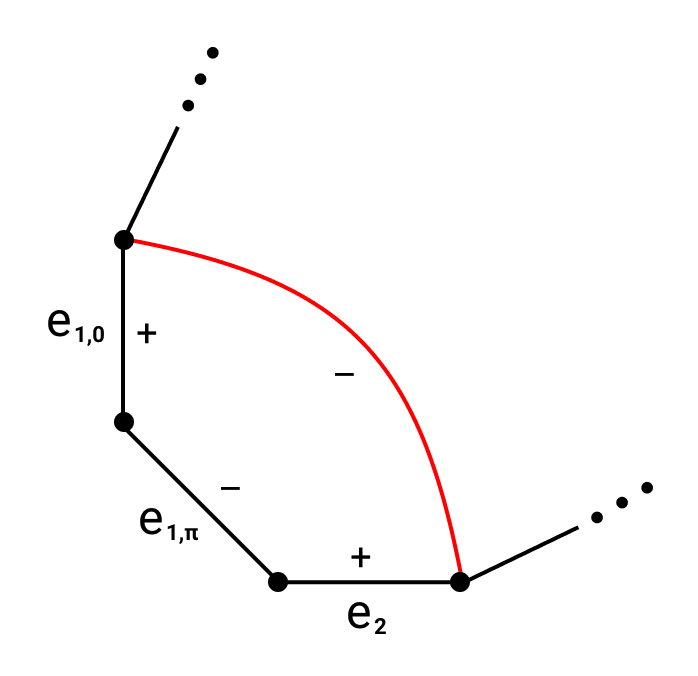
\includegraphics[width=5cm]{more_pictures/one_edge.png}
%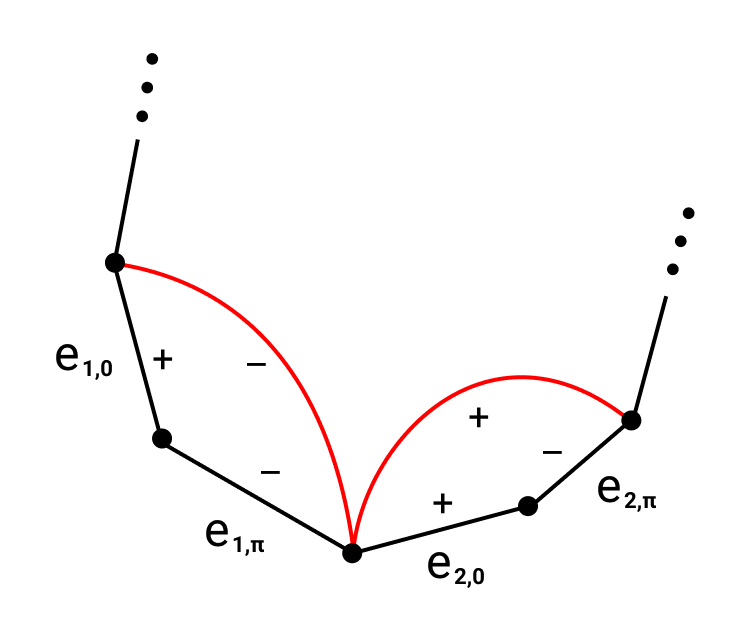
\includegraphics[width=5cm]{more_pictures/two_edge.png}
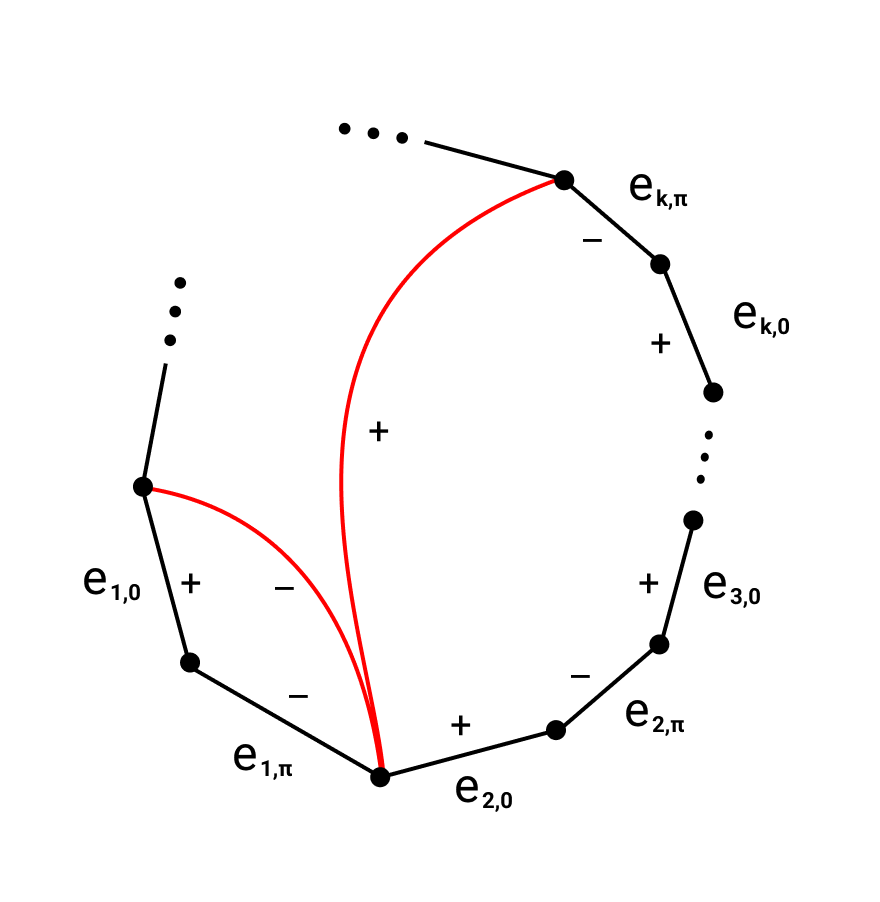
\includegraphics[width=5cm]{more_pictures/two_edge_many.png}
\caption{Red edge indicates an added edge to the graph to appropriately assign +/- labels which indicate 
increasing/decreasing angles on the edge respectively.}
\label{f:adding_edges}
\end{figure}

Now we deform the $\theta^*$ based on Figure \ref{f:adding_edges},
increasing/decreasing by some small $\veps' > 0$ if the edge
is labeled $+/-$.
Note some edges may be labeled twice, in which case we perform
both increasing/decreasing (e.g. if it is labeled $+$ and $-$,
the $\theta^*$ is not changed).
It is easy to see that the sum of $\theta^*$ around a vertex
remains unchanged.
Furthermore, all the edges with $\theta^*$ originally equal 0,
i.e. all $e_{i,0}$'s,
now have positive $\theta^*$,
(it receives only one label $+$,
because the other face it meets is a bow-tie).



%Thus, we could attempt to apply the feasible flow theorem in a similar manner,
%and obtain an angle-splitting for $\sT_T(L)'$, but 
%TODO rephrase nicely.
We can directly get an angle-splitting for $\sT_T(L)'$
using the angle-splitting for $\sT_T(L)$.
We reuse the $+/-$ assignments from Figure \ref{f:adding_edges}.
For $e = e_{i,0}$, we increase $\vphi_{\vec{e}}, \vphi_{\cev{e}}$
by $\veps'/2$ each; for $e = e_{i,\pi}$,
we decrease them by $\veps'/2$ each.
For other edges, we increase/decrease $\vphi_{\vec{e}}$ by $\veps'$,
where $\vec{e}$ is the oriented edge corresponding to the side
on which the $+/-$ sign appears in Figure \ref{f:adding_edges};
so for example, if an edge $e$ receives both $+$ and $-$,
then one of $\vphi_{\vec{e}},\vphi_{\cev{e}}$ increases
while the other decreases, thus $\theta_e^*$ remains constant.


Now we address $\sT_B(L)$.
In the gluing of $\sT_T(L)$ to $\sT_B(L)$,
non-bow-tie faces of $\Gamma_T(L)$ are identified with
non-bow-tie faces of $\Gamma_B(L)$.
Under this identification, we add the same edges to $\Gamma_B(L)$,
thus obtaining the new torihedron $\sT_B(L)'$ with graph
$\Gamma_B(L)'$.
We perform the same deformations of $\theta^*$'s (or $\vphi$'s).


We need to check that upon gluing $\sT_T(L)'$ to $\sT_B(L)'$,
the sum of dihedral angles around each edge is still $2\pi$.
This was clearly true before deforming, as the new edges of
$\Gamma_T(L)'$ only gets identified with the unique
corresponding edge of $\Gamma_B(L)'$, and they are both labeled
with $\theta^* = \pi$.
To see that the deformation does not change these sums,
note that in the identification of faces of $\Gamma_T(L)'$
to $\Gamma_B(L)'$,
an edge with $\theta^*=0$ is identified with an edge with
$\theta^*=\pi$,
so an increase in the former would be conterbalanced by
a decrease in the latter.
It is also easy to see this is the case for the other edges.
(Once again, a similar argument applies if $\sT_T(L)'$
and $\sT_B(L)'$ are glued assuming
some augmentations had no half-twist;
see end of proof where we deal with $K$ having bigons.)
%see \remref{r:nohalftwist}.)


Finally, for each face of $\Gamma_T(L)'$ that has more than three sides,
we arbitrarily decompose it into triangles
and apply \lemref{l:pyramid_decomp}
to obtain a triangulation of $\sT_T(L)'$ into non-degenerate angled tetrahedra;
perform the corresponding decomposition for faces of
$\Gamma_B(L)'$ and obtain a triangulation of $\sT_B(L)'$
into non-degenerate angled tetrahedra.
Upon gluing, this gives an angle structure on the triangulation
of $\toruscomp{L}$


Now let us consider $K$ with bigons.
Let $K'$ be the link obtained from $K$ by replacing
each twist region of $K$ by a single appropriate crossing.
Let $L'$ be the link obtained from augmenting $K'$
by exactly the same crossing circles.
The top and bottom torihedra $\sT_T(L'),\sT_B(L')$
are the same as $\sT_T(L),\sT_B(L)$;
however, the gluing differs slightly:
for twist regions of $K$ that have an even number of bigons,
the gluing of $\sT_T(L')$ to $\sT_B(L')$
should be using Figure \ref{fig:falGluings} (a) (not (b)).
As remarked throughout the proof,
all the arguments carry through verbatim.

%Then the only difference in the arguments
%is that, for twist regions of $K$ that have an even number of bigons,
%the 

%\begin{remark}
%\label{r:nohalftwist}
If the original link $K$ had some twist regions with at least one bigon,
we may consider augmentations $L$ where all such twist regions
are augmented, i.e. $L$ may have augmentations without half-twists.
Then, as pointed out in proof of \thmref{t:auglink_hyp} above,
the proof still works for $L$, showing that $L$ is also hyperbolic.
%\end{remark}


\end{proof}


\bibliographystyle{plain}
\bibliography{references-ak}


\end{document}
